\documentclass[12pt]{article}
%--------------------   start of the 'preamble'
%
\usepackage{graphicx,amssymb,amstext,amsmath,color}
\usepackage{grffile}
\usepackage[margin=2cm]{geometry}
\usepackage{abstract}
\usepackage{setspace}
\usepackage[footnotesize,bf]{caption}

% TABLE
\usepackage{multicol,hhline,colortbl,multirow}
\usepackage{braket}
\usepackage{siunitx}
\usepackage{hyperref}
\usepackage{authblk}
\usepackage{siunitx}
\usepackage{adjustbox}
\usepackage{mathrsfs}
%%\usepackage[sort&compress]{natbib}
%%\bibpunct{(}{)}{,}{a}{, }{;}
%
\usepackage[sort&compress]{natbib}
\bibpunct{[}{]}{,}{s}{}{;}


\definecolor{gray}{gray}{0.8}
\def\mobunits{\square\centi\meter\per\volt\per\second}
\def\gcm{\gram\per\cubic\centi\meter}
\def\ccg{\cellcolor{gray}}

\renewcommand{\labelitemii}{$\circ$}
\renewcommand{\bibname}{References}


\title{MorphCT Results - Equilibration Sensitivity}
\author{Matthew Jones}
\date{\today}

\begin{document}
\maketitle

\section{Preface}

%This document describes the results obtained during `AIChE week' 2017.
%There are lots of different things being explored simultaneously, so I'll try and explain what each set of results pertains to.
I spent a while updating and improving our plotting subroutines.
The graphs look mostly the same, but \textcolor{red}{I will be no longer using bold numbers to indicate morphology types, and figures will no longer be organised by plot type (i.e. hopping rate, network, etc.) with each panel corresponding to a different morphology.}
To get a better idea of the differences between plots, each figure will be one page describing one morphology completely, with each panel showing a different plot type for that morphology.
This makes it easier to open windows side by side and get the complete morphology picture.
It also has the advantage of the plotting being completely automated, dramatically reducing labour time generating the figures.


\section{What effect does fully equilibrating after fine-graining have on the charge transport properties?}


\subsection{Explanation}


I took the pristine P3HT results that we had previously (using the Voronoi cells for neighbour calculations) and compared them to systems that were equilibrated for a long time during the final MD phase of the molecular dynamics process.
The final MD phase of the `Unequilibrated' systems ran for 1E5 timesteps, whereas the `equilibrated' systems were run for 1E7 timesteps instead.
Figure \ref{fig:Energy} shows the potential energy evolution for the T = 1.5 system.


\begin{figure}[h!]\centering
	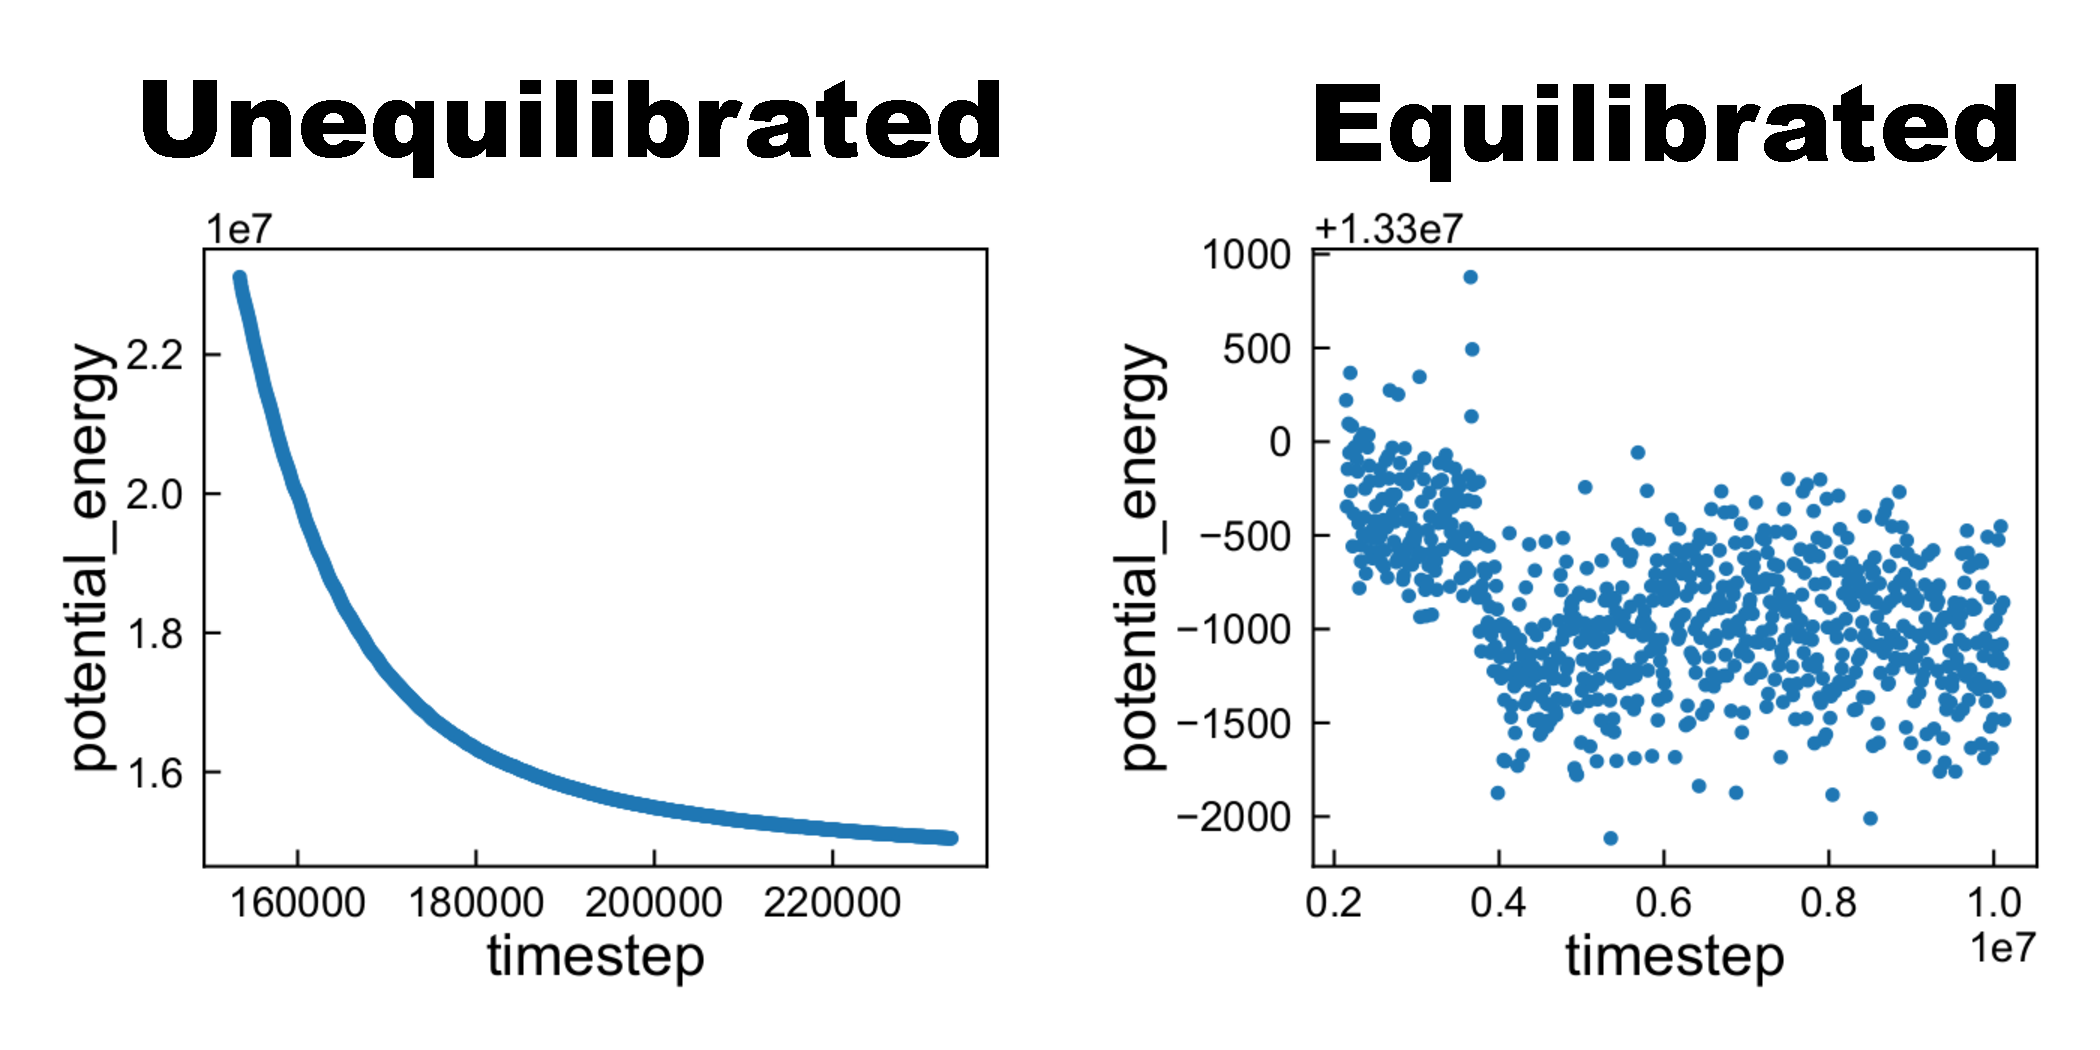
\includegraphics[width=\textwidth]{Figures/PE.pdf}
    \caption{The evolution of the total potential energy for the p1-L15-f0.0-P0.1-T1.5-e0.5 systems.
    a) The original `unequilibrated' system, where the final MD phase ran for 1E5 timesteps.
    b) The new `equilibrated' system, where the final MD phase ran for 1E7 timesteps.
    In both cases, the potential energy was dumped 1000 times, so there were 100 timesteps between each energy value in the unequilibrated case, and 10,000 timesteps in the equilibrated case.
    Only the final 800 energy values recorded are shown here.}
	\label{fig:Energy}
\end{figure}


Figure \ref{fig:Mobility} shows the mobility curve differences between the two systems.


\begin{figure}[h!]\centering
	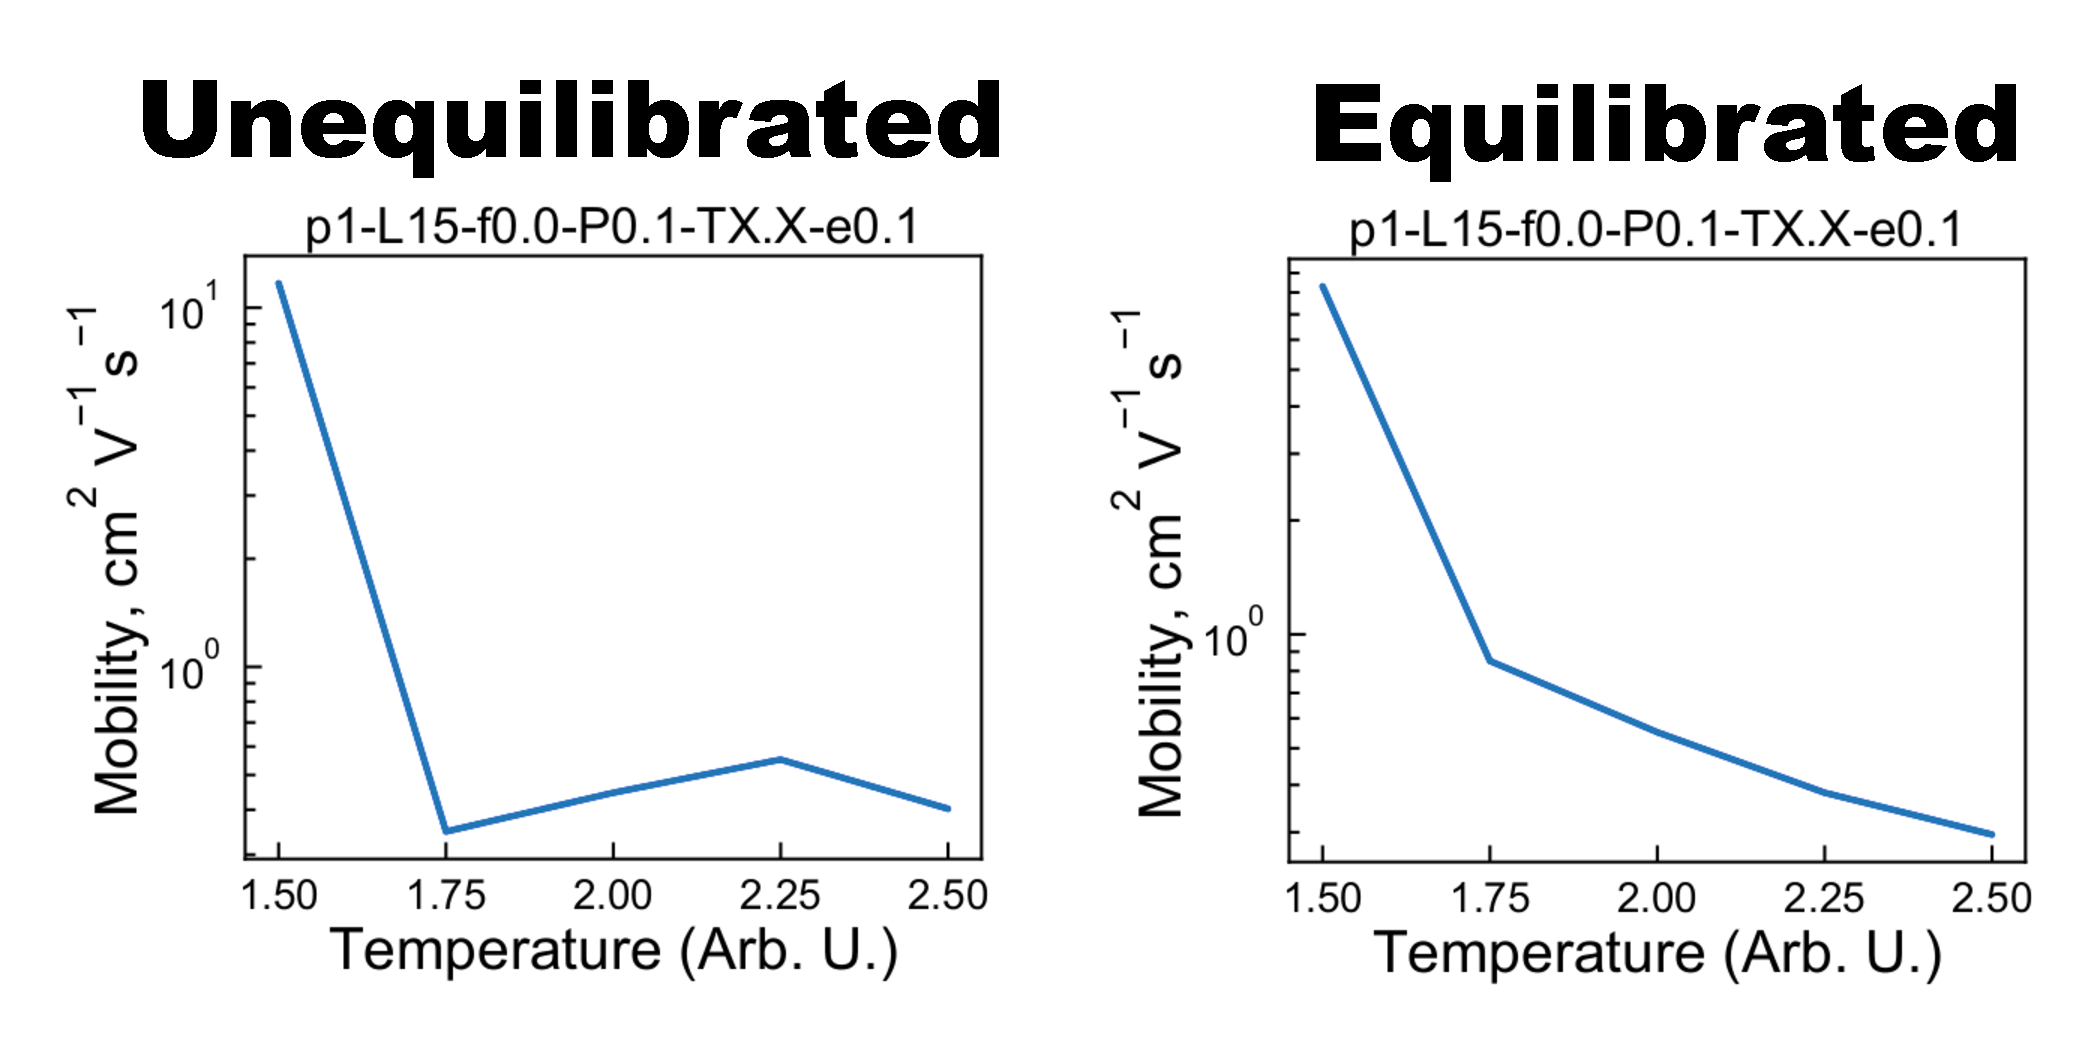
\includegraphics[width=\textwidth]{Figures/Mob.pdf}
    \caption{The evolution of the mobility for the neat P3HT state points.
    a) The original `unequilibrated' system, where the final MD phase ran for 1E5 timesteps.
    b) The new `equilibrated' system, where the final MD phase ran for 1E7 timesteps.
}
	\label{fig:Mobility}
\end{figure}


The mobility trend has somewhat washed out, as there is now a smaller difference between the ordered and the disordered morphologies.
Additionally, there is now a more obvious decrement in mobility as a function of system temperature, allowing for some distinction between the disordered systems.
The absolute values however are largely the same as previously, with less than an order of magnitude difference between them.


\subsection{Dependence of Equilibration on Tau}


\begin{figure}[h!]\centering
	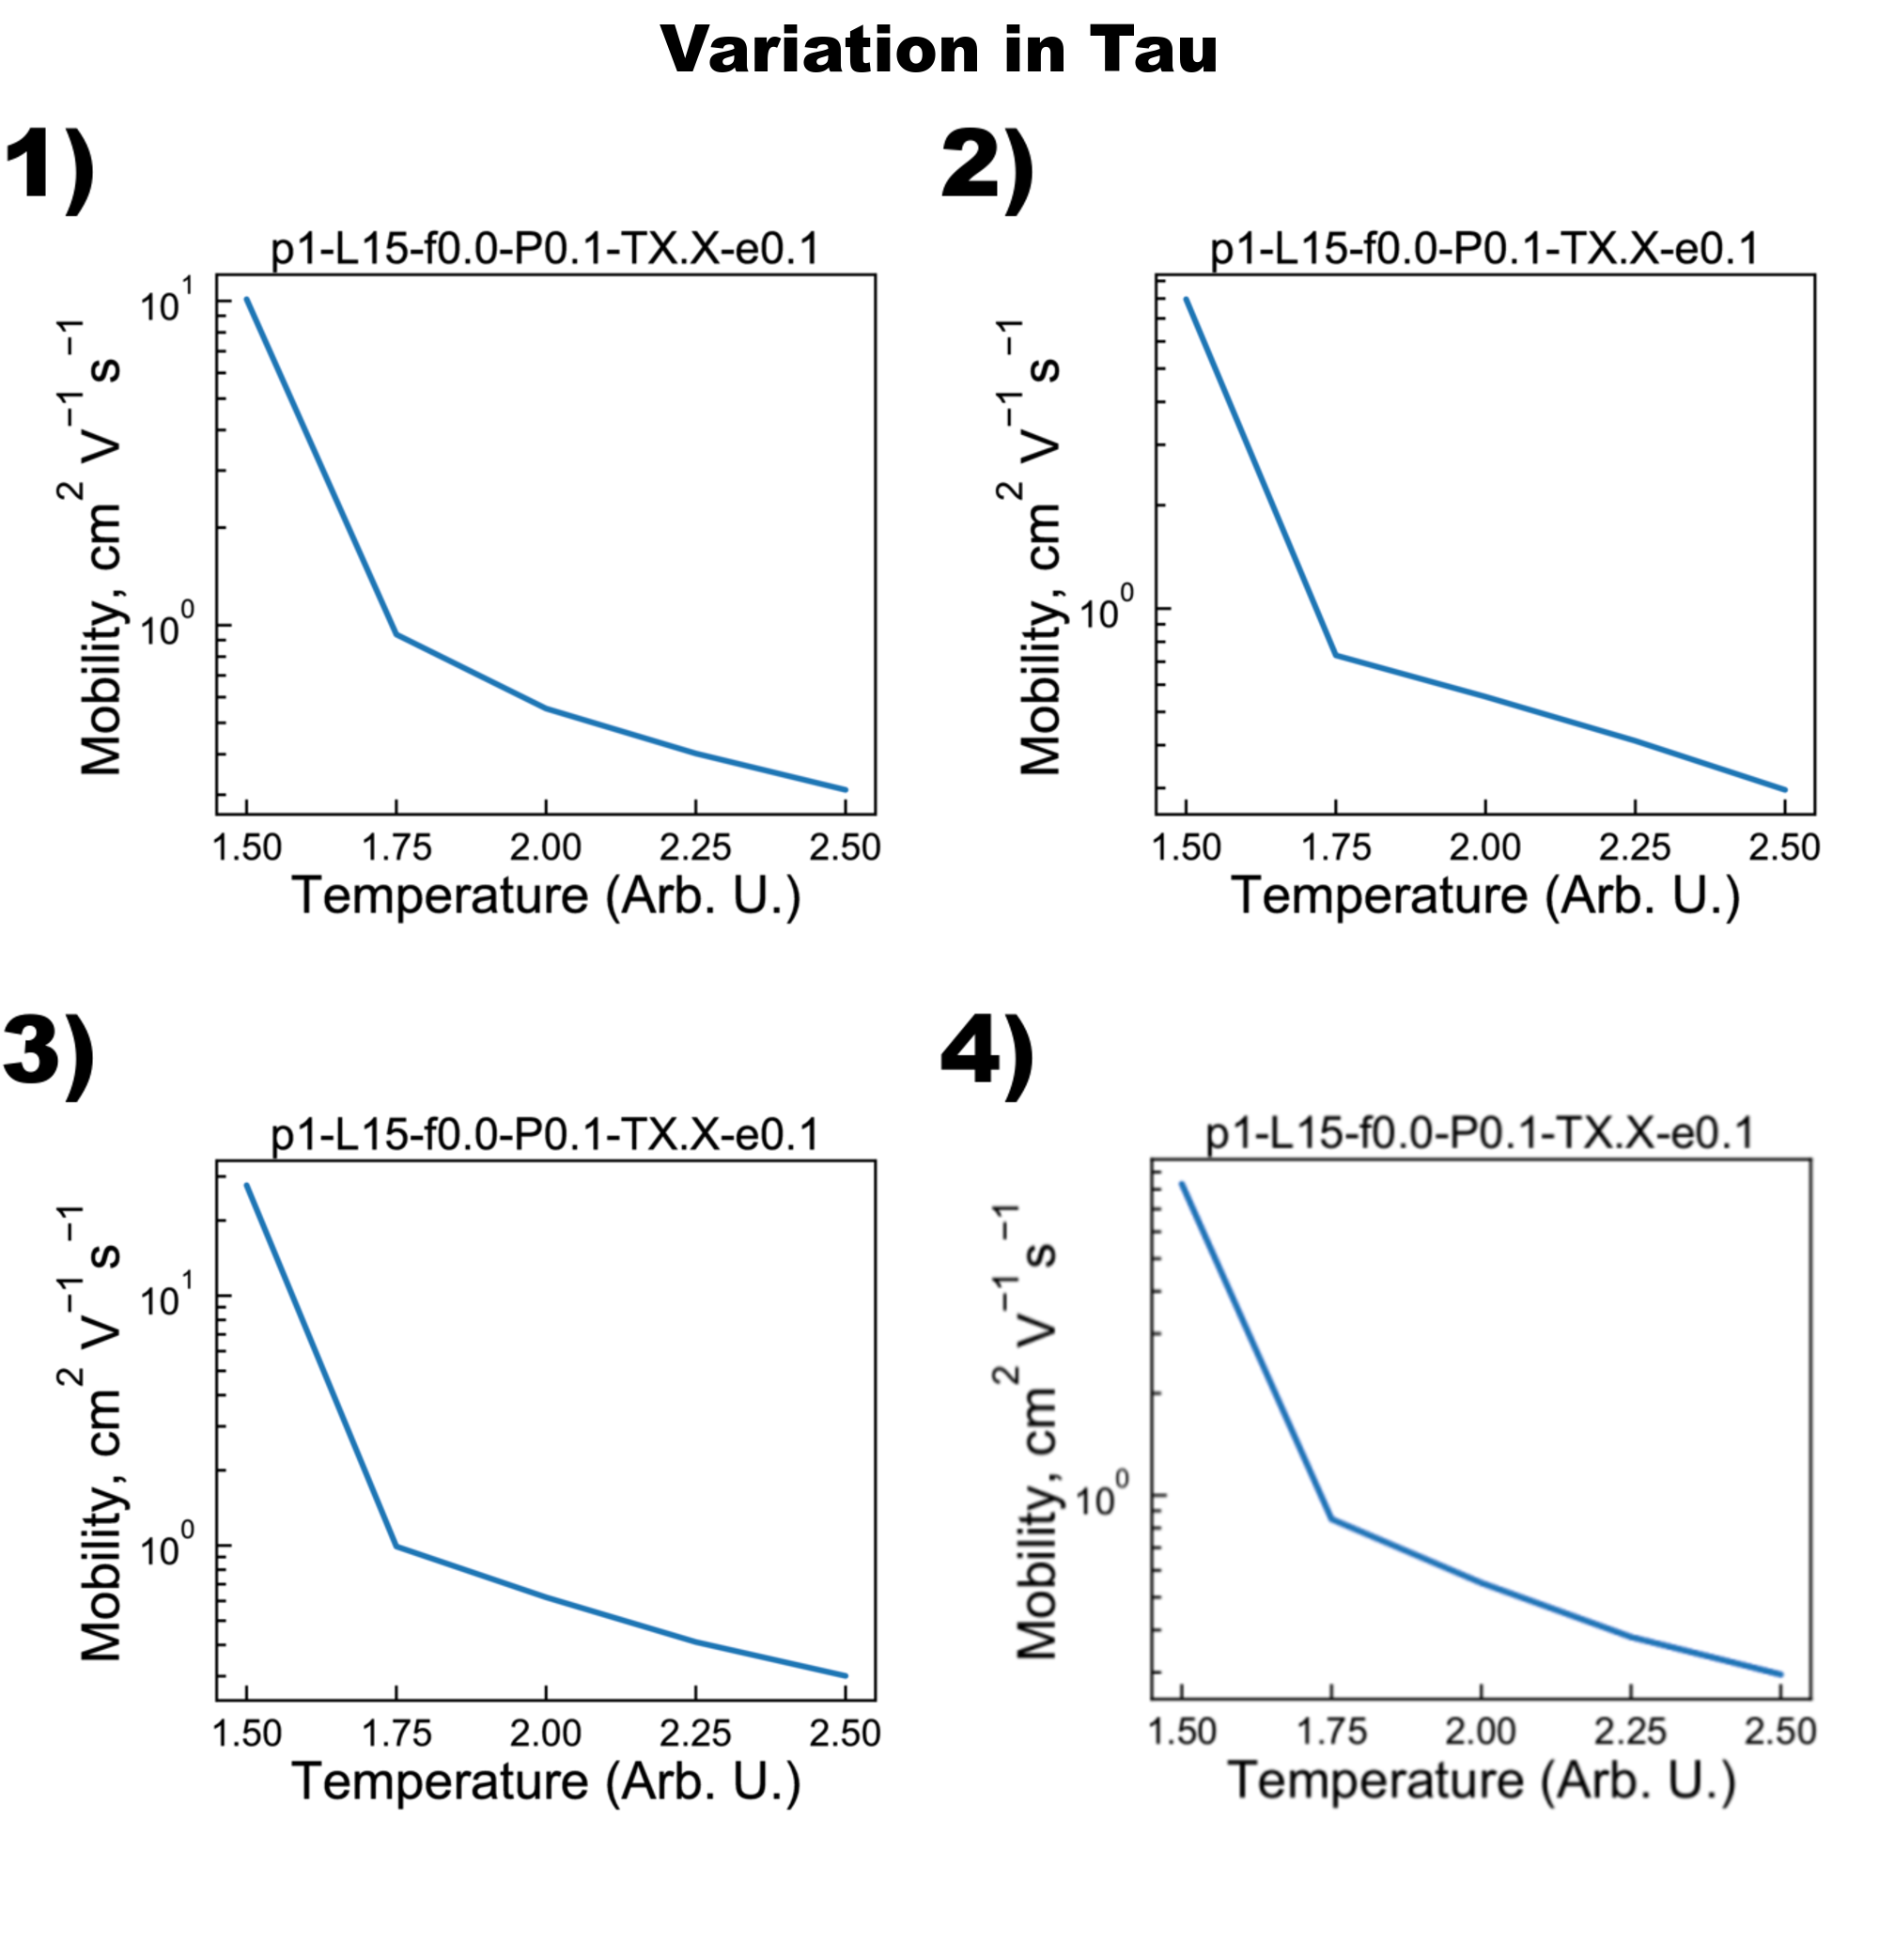
\includegraphics[width=\textwidth]{Figures/Variation_in_Tau.png}
    \caption{The mobilities for systems that have been equilibrated with varying values of thermostat coupling, $\tau$:
    1) $\tau = 0.5$,
    2) $\tau = 1.0$,
    3) $\tau = 5.0$,
    4) $\tau = 10.0$}
	\label{fig:Tau}
\end{figure}


As can be seen, there is no substantial difference between the absolute values of mobility, nor the order-disorder trend as a function of $\tau$.
There is a slight `washing out' of the trend that describes the difference between the ordered and disordered systems - the mobility at $T = 1.5$ is about a factor of 10x greater than $T = 1.75$, at $\tau = 0.5$, which increases to a factor of 14x at $\tau = 5.0$.

\textcolor{red}{For completeness, I am running the 5 jobs again, this time regenerating the atom velocities based on a normal distribution and the input temperature between each molecular dynamics phase.
These results will be added to this summary when the jobs finish.}

\clearpage

\subsection{Original (Unequilibrated) Results}


\begin{figure}[h]\centering
	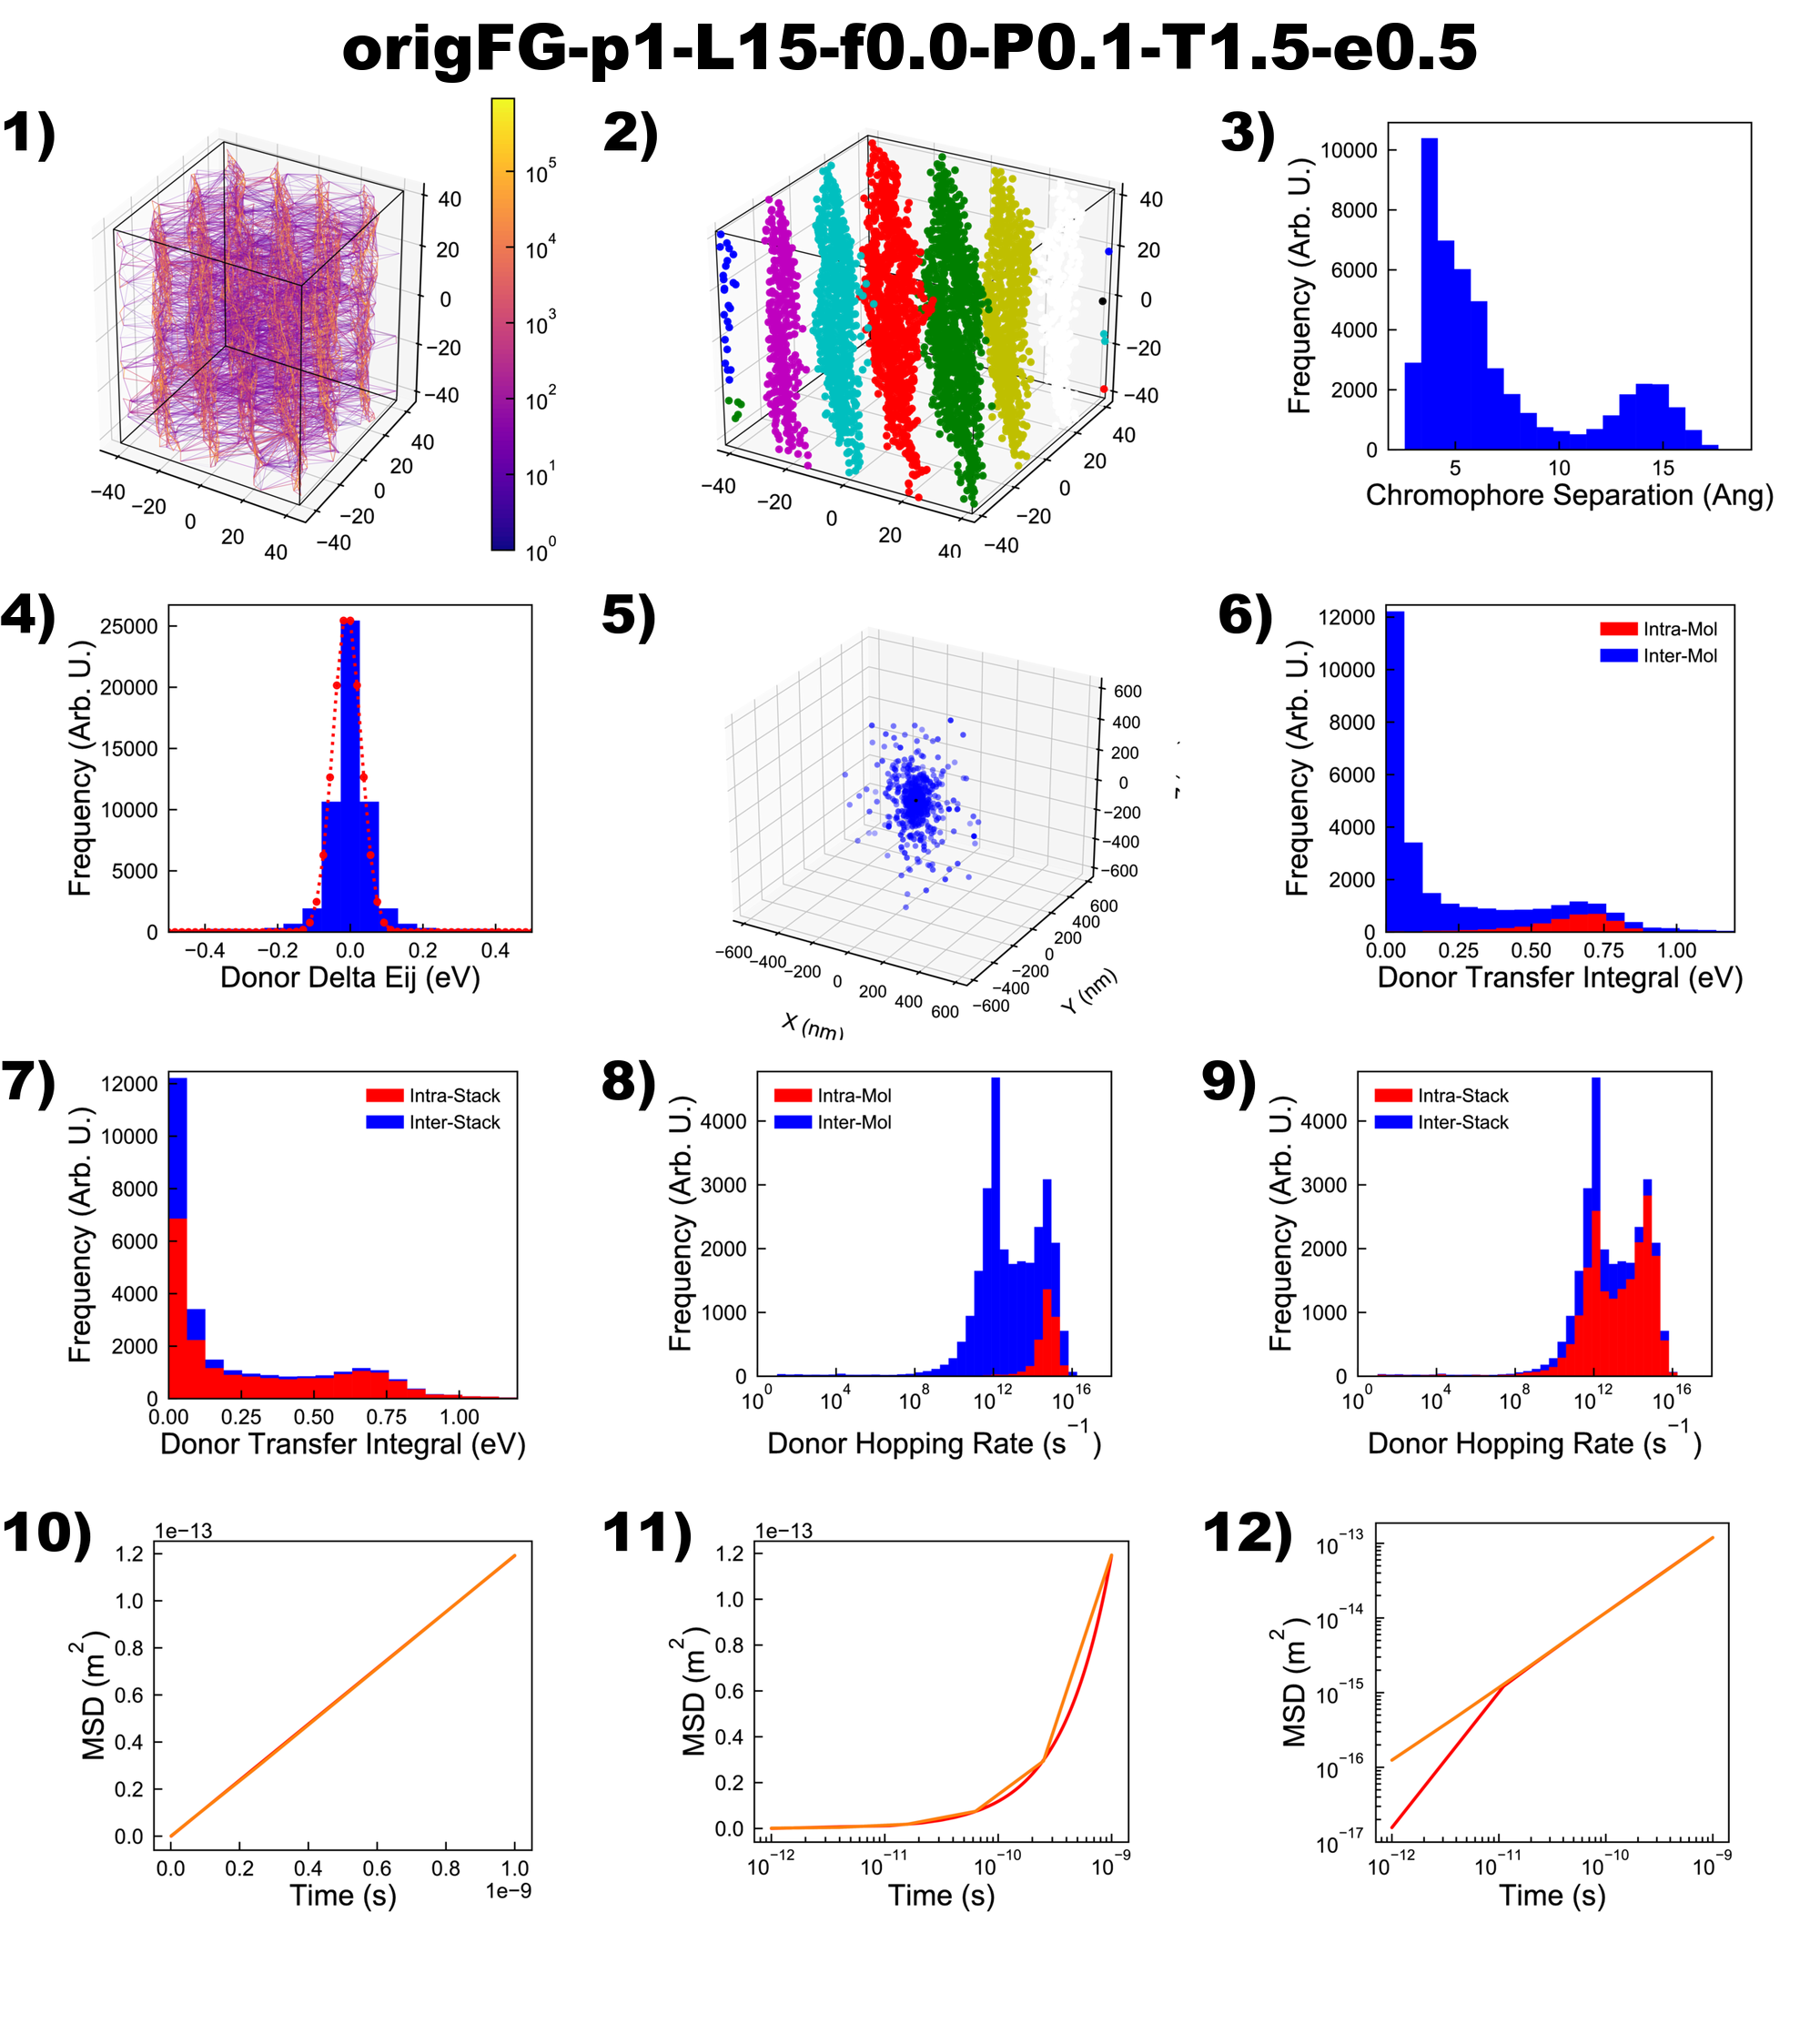
\includegraphics[width=0.8\textwidth]{Figures/origFG-p1-L15-f0.0-P0.1-T1.5-e0.5.png}
    \caption{   1) Chromophore connectivity network, 
                2) Location of `stacks', 
                3) Distribution of connected chromophore separations (defines stacks),
                4) Density of states of Frontier molecular orbital (delta Eij),
                5) KMC Carrier termination locations (defines anisotropy),
                6) Histogram of molecular transfer integrals,
                7) Histogram of stack transfer integrals,
                8) Histogram of molecular hopping rates,
                9) Histogram of stack hopping rates,
                10) Linear MSD plot,
                11) Semi-log-x MSD plot,
                12) Logarithmic MSD plot.}
	\label{fig:UneqlT1.5}
\end{figure}


\begin{figure}[h]\centering
	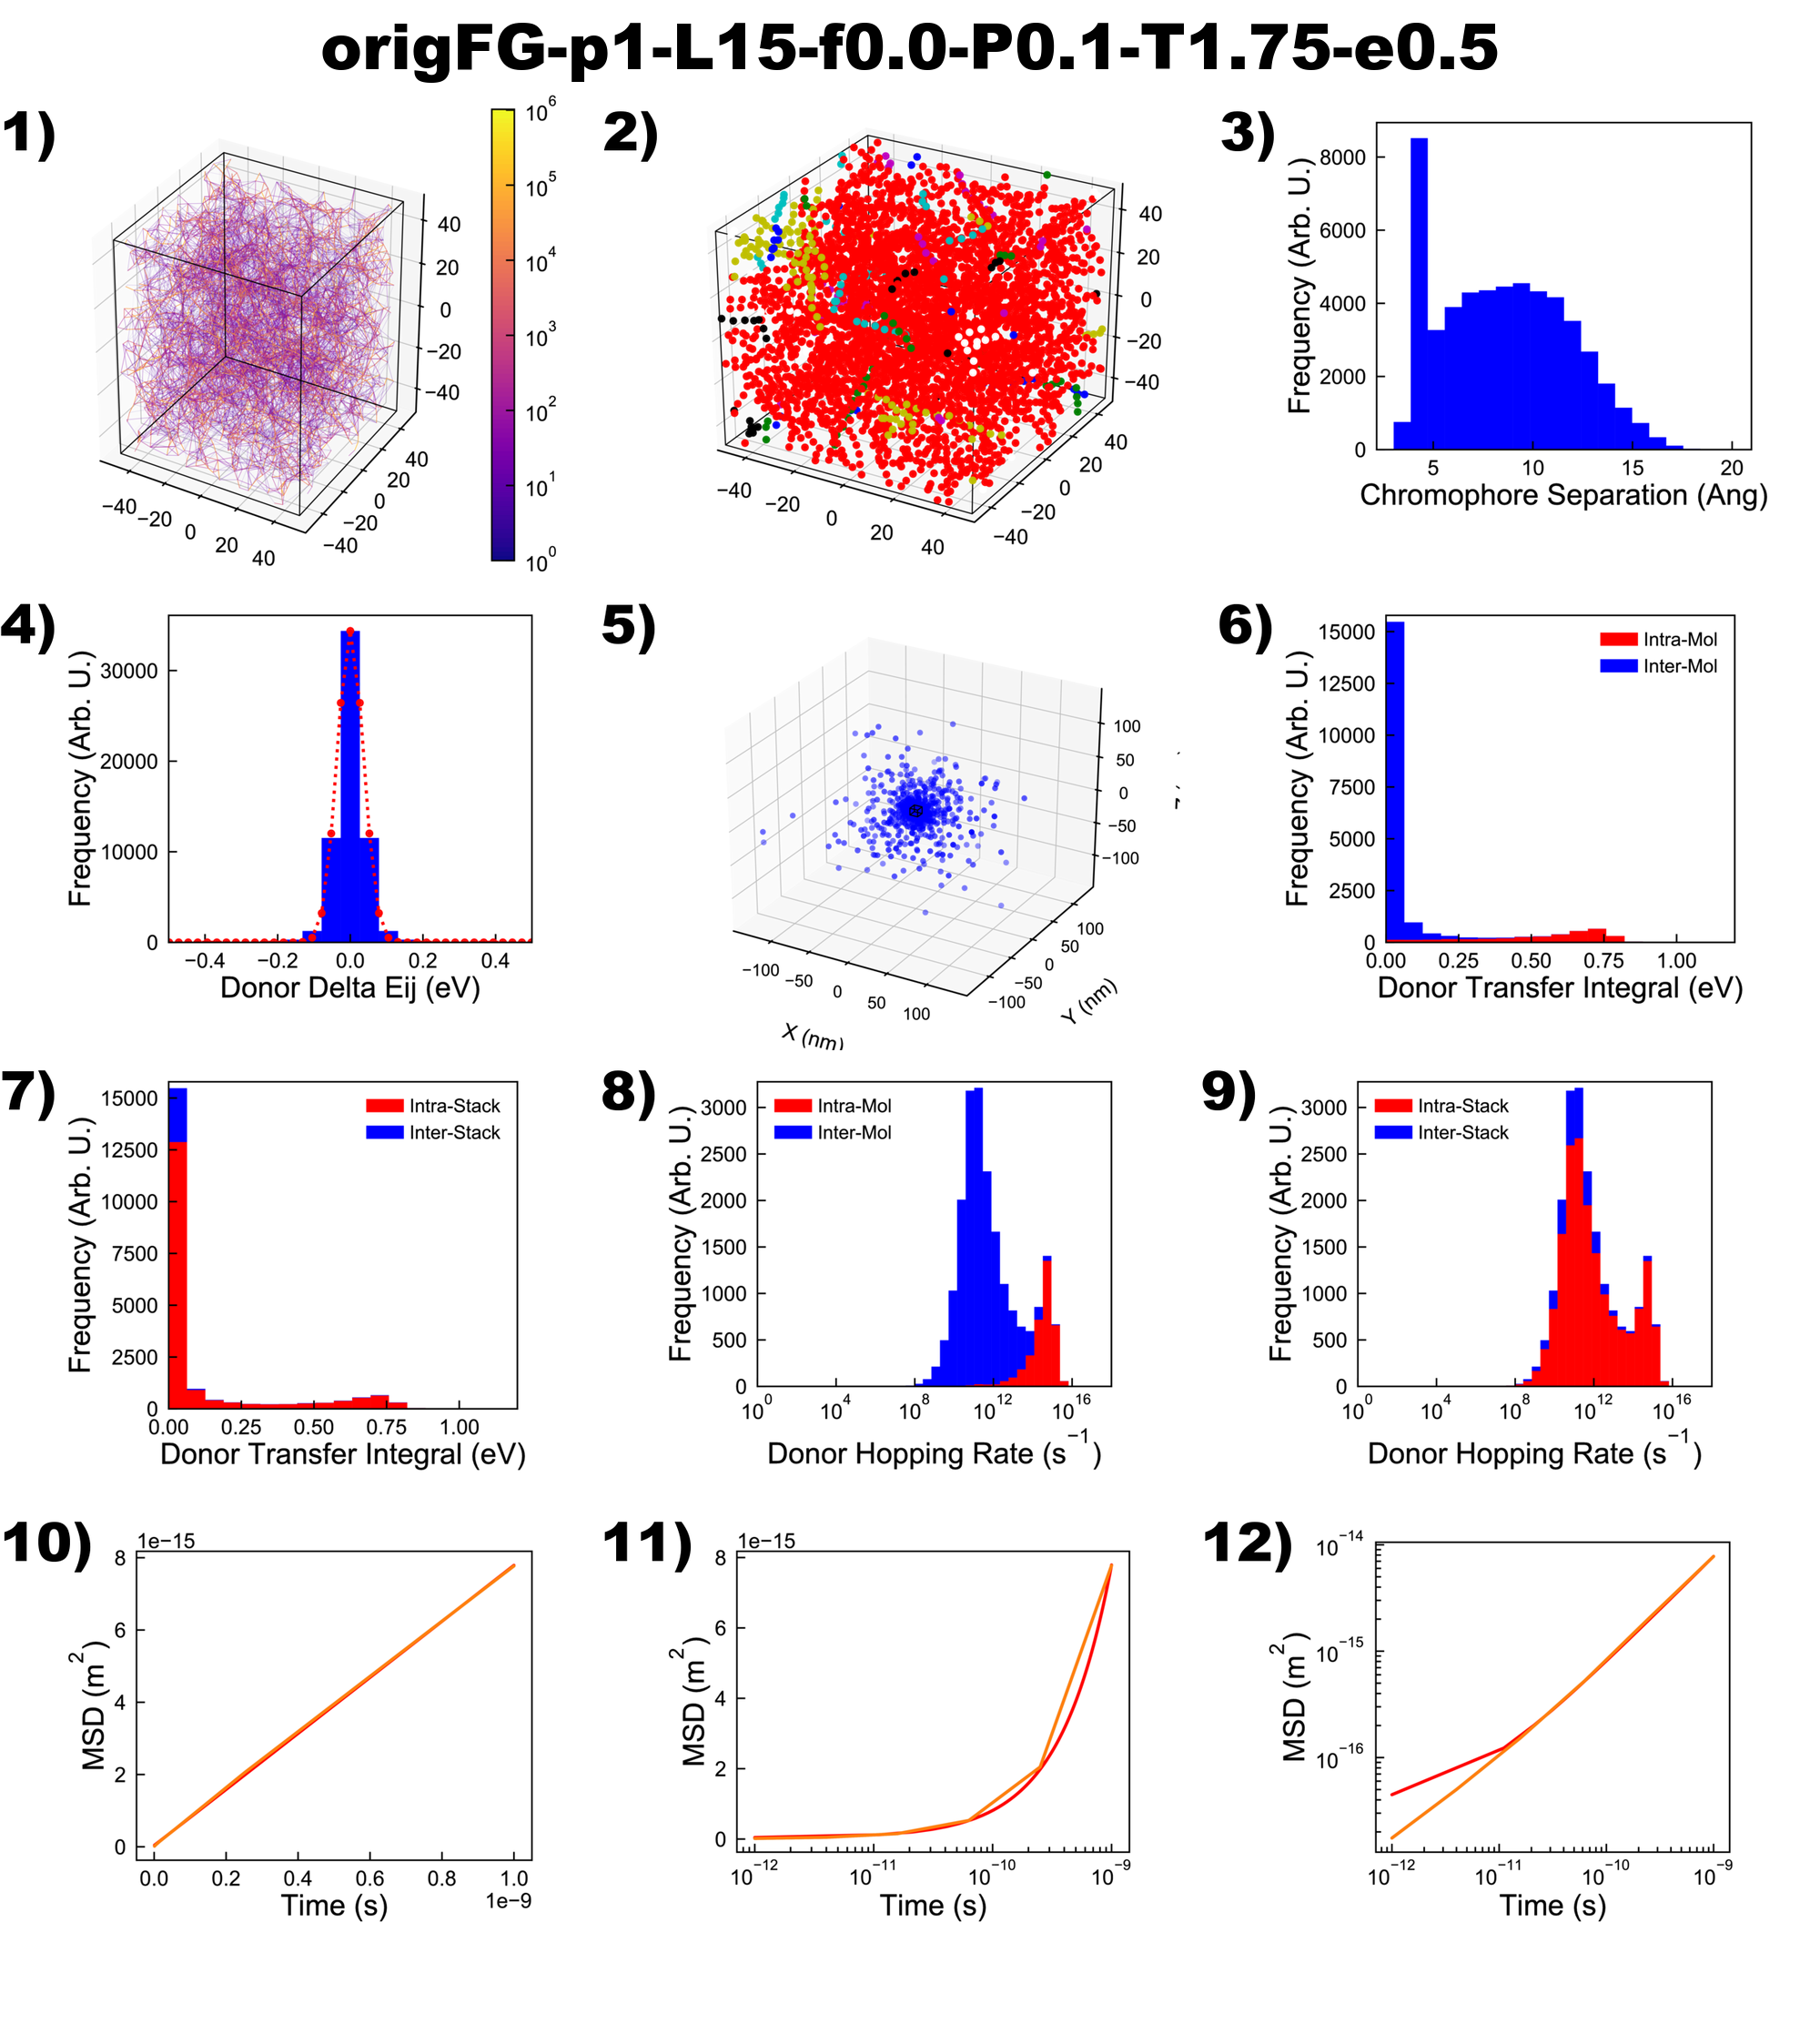
\includegraphics[width=\textwidth]{Figures/origFG-p1-L15-f0.0-P0.1-T1.75-e0.5.png}
    \caption{   1) Chromophore connectivity network, 
                2) Location of `stacks', 
                3) Distribution of connected chromophore separations (defines stacks),
                4) Density of states of Frontier molecular orbital (delta Eij),
                5) KMC Carrier termination locations (defines anisotropy),
                6) Histogram of molecular transfer integrals,
                7) Histogram of stack transfer integrals,
                8) Histogram of molecular hopping rates,
                9) Histogram of stack hopping rates,
                10) Linear MSD plot,
                11) Semi-log-x MSD plot,
                12) Logarithmic MSD plot.}
	\label{fig:UneqlT1.75}
\end{figure}


\begin{figure}[h]\centering
	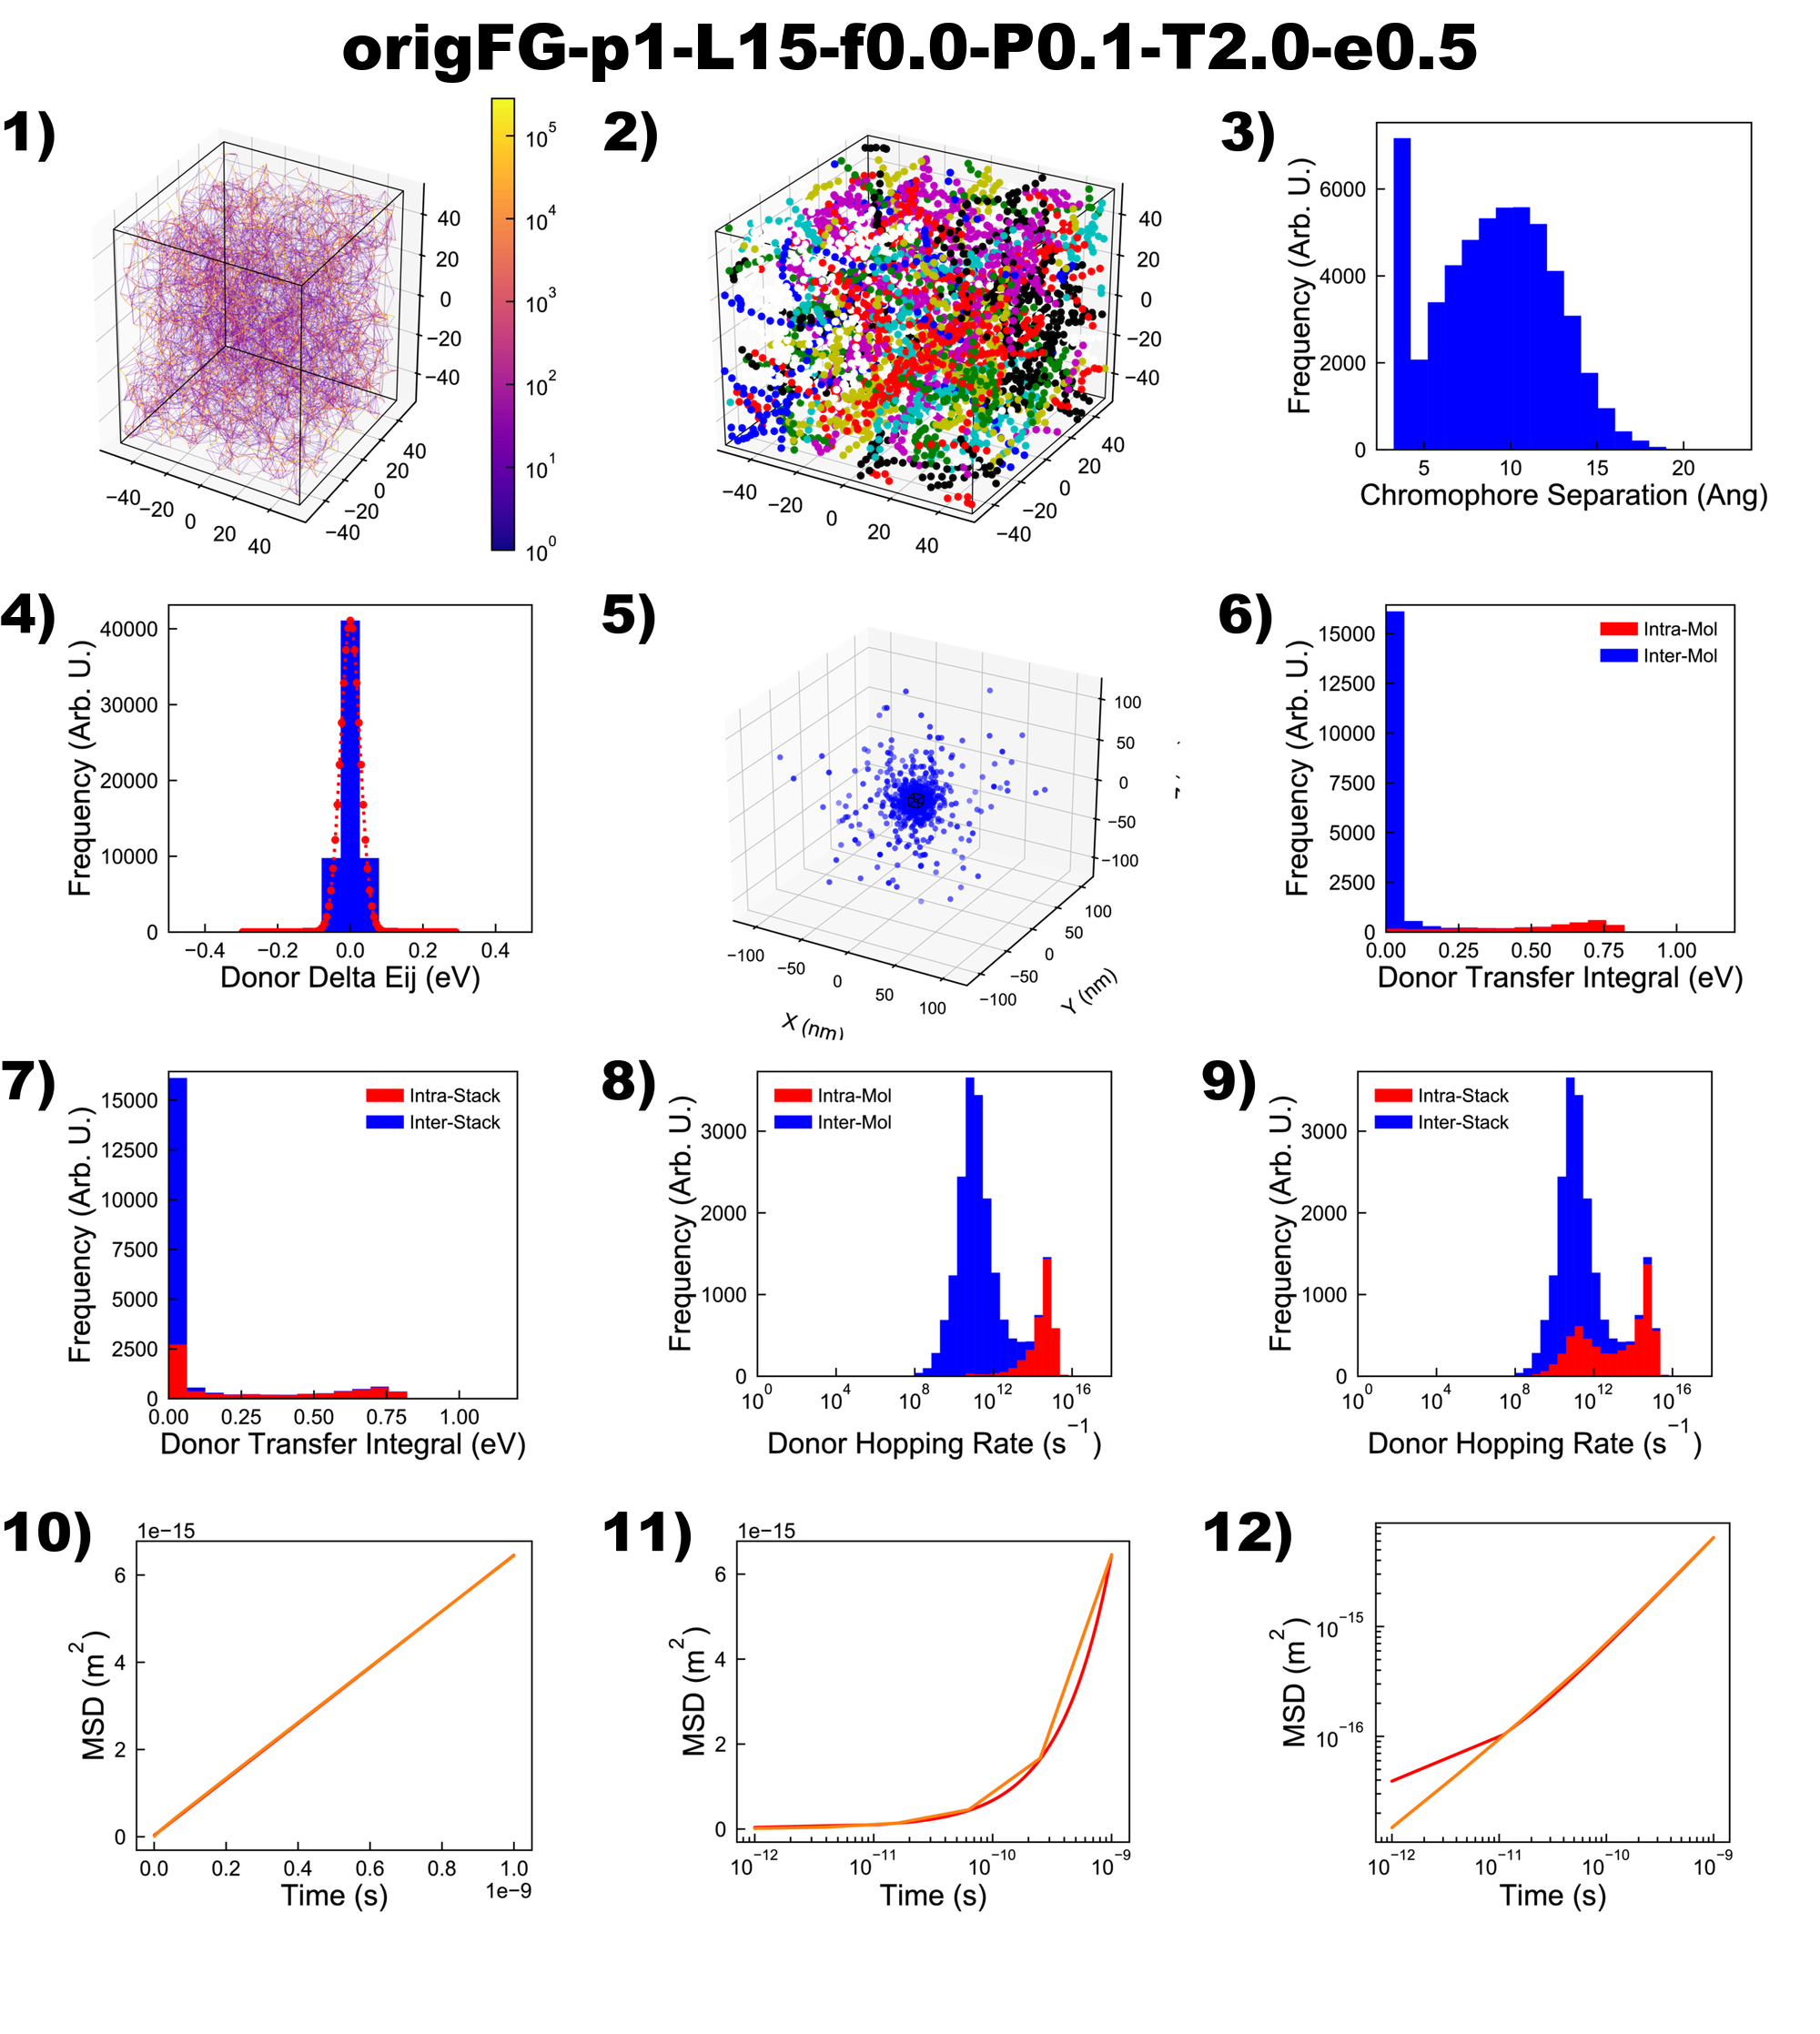
\includegraphics[width=\textwidth]{Figures/origFG-p1-L15-f0.0-P0.1-T2.0-e0.5.png}
    \caption{   1) Chromophore connectivity network, 
                2) Location of `stacks', 
                3) Distribution of connected chromophore separations (defines stacks),
                4) Density of states of Frontier molecular orbital (delta Eij),
                5) KMC Carrier termination locations (defines anisotropy),
                6) Histogram of molecular transfer integrals,
                7) Histogram of stack transfer integrals,
                8) Histogram of molecular hopping rates,
                9) Histogram of stack hopping rates,
                10) Linear MSD plot,
                11) Semi-log-x MSD plot,
                12) Logarithmic MSD plot.}
	\label{fig:UneqlT2.0}
\end{figure}


\begin{figure}[h]\centering
	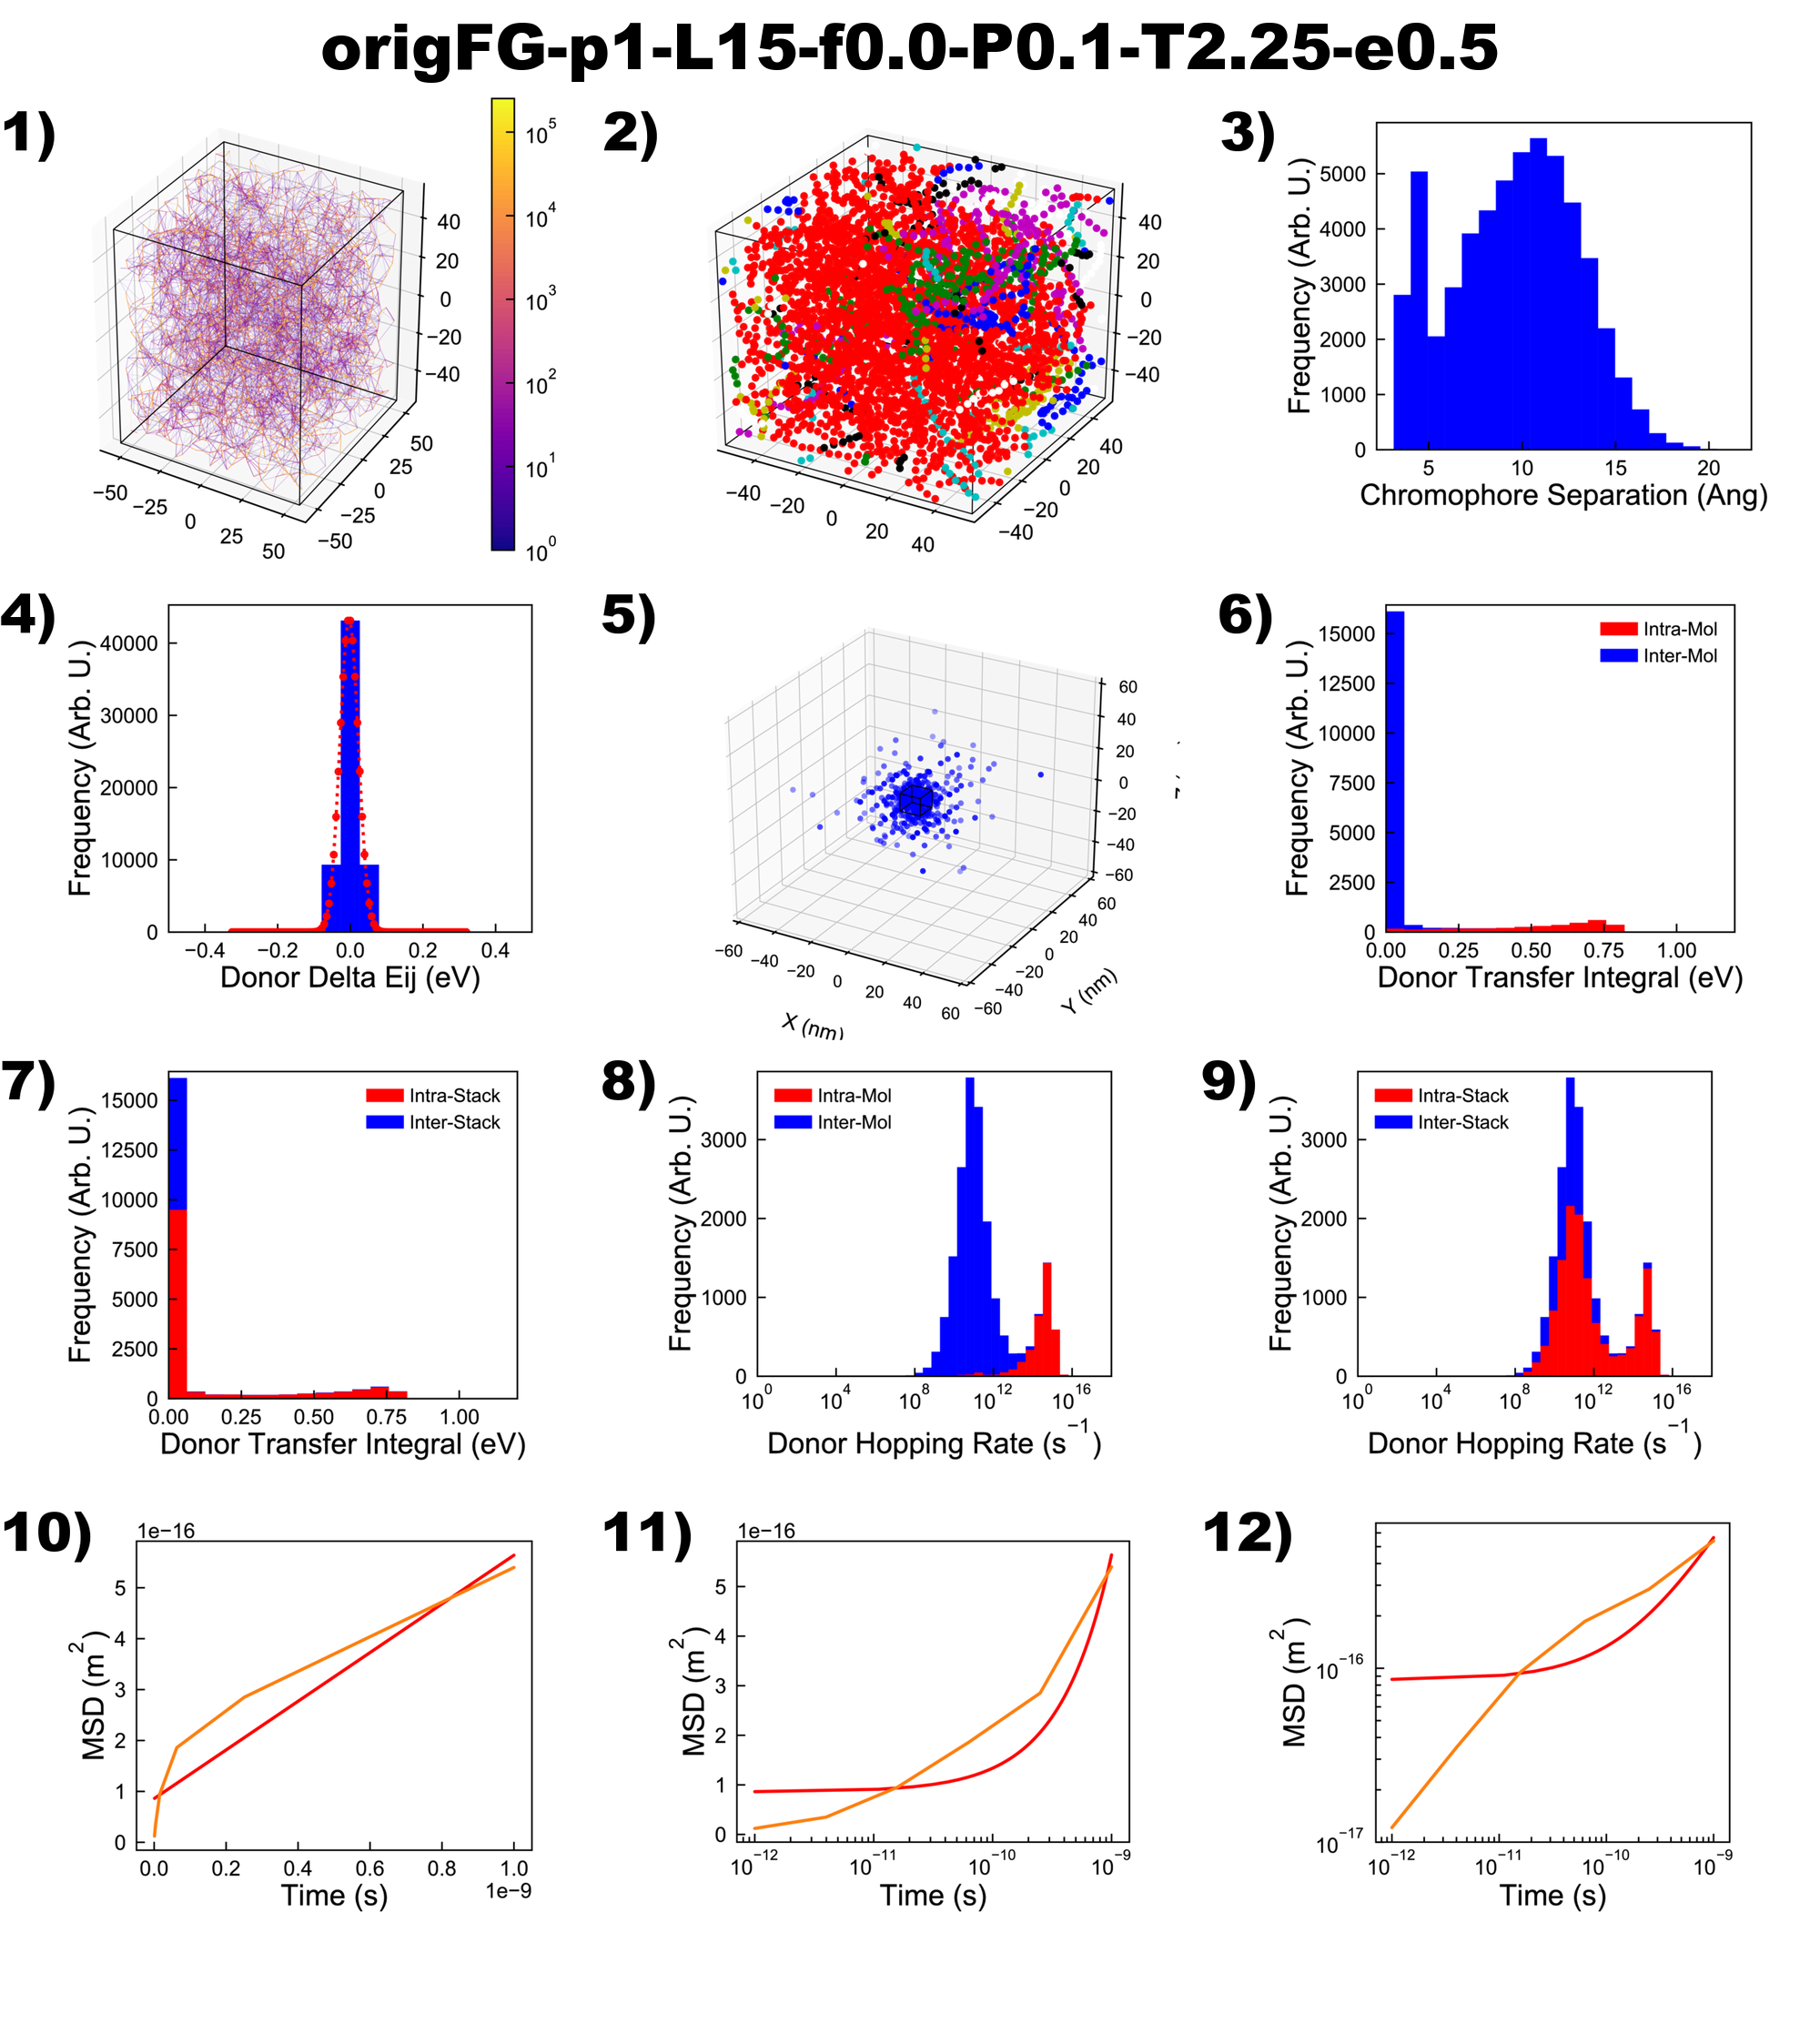
\includegraphics[width=\textwidth]{Figures/origFG-p1-L15-f0.0-P0.1-T2.25-e0.5.png}
    \caption{   1) Chromophore connectivity network, 
                2) Location of `stacks', 
                3) Distribution of connected chromophore separations (defines stacks),
                4) Density of states of Frontier molecular orbital (delta Eij),
                5) KMC Carrier termination locations (defines anisotropy),
                6) Histogram of molecular transfer integrals,
                7) Histogram of stack transfer integrals,
                8) Histogram of molecular hopping rates,
                9) Histogram of stack hopping rates,
                10) Linear MSD plot,
                11) Semi-log-x MSD plot,
                12) Logarithmic MSD plot.}
	\label{fig:UneqlT2.25}
\end{figure}


\begin{figure}[h]\centering
	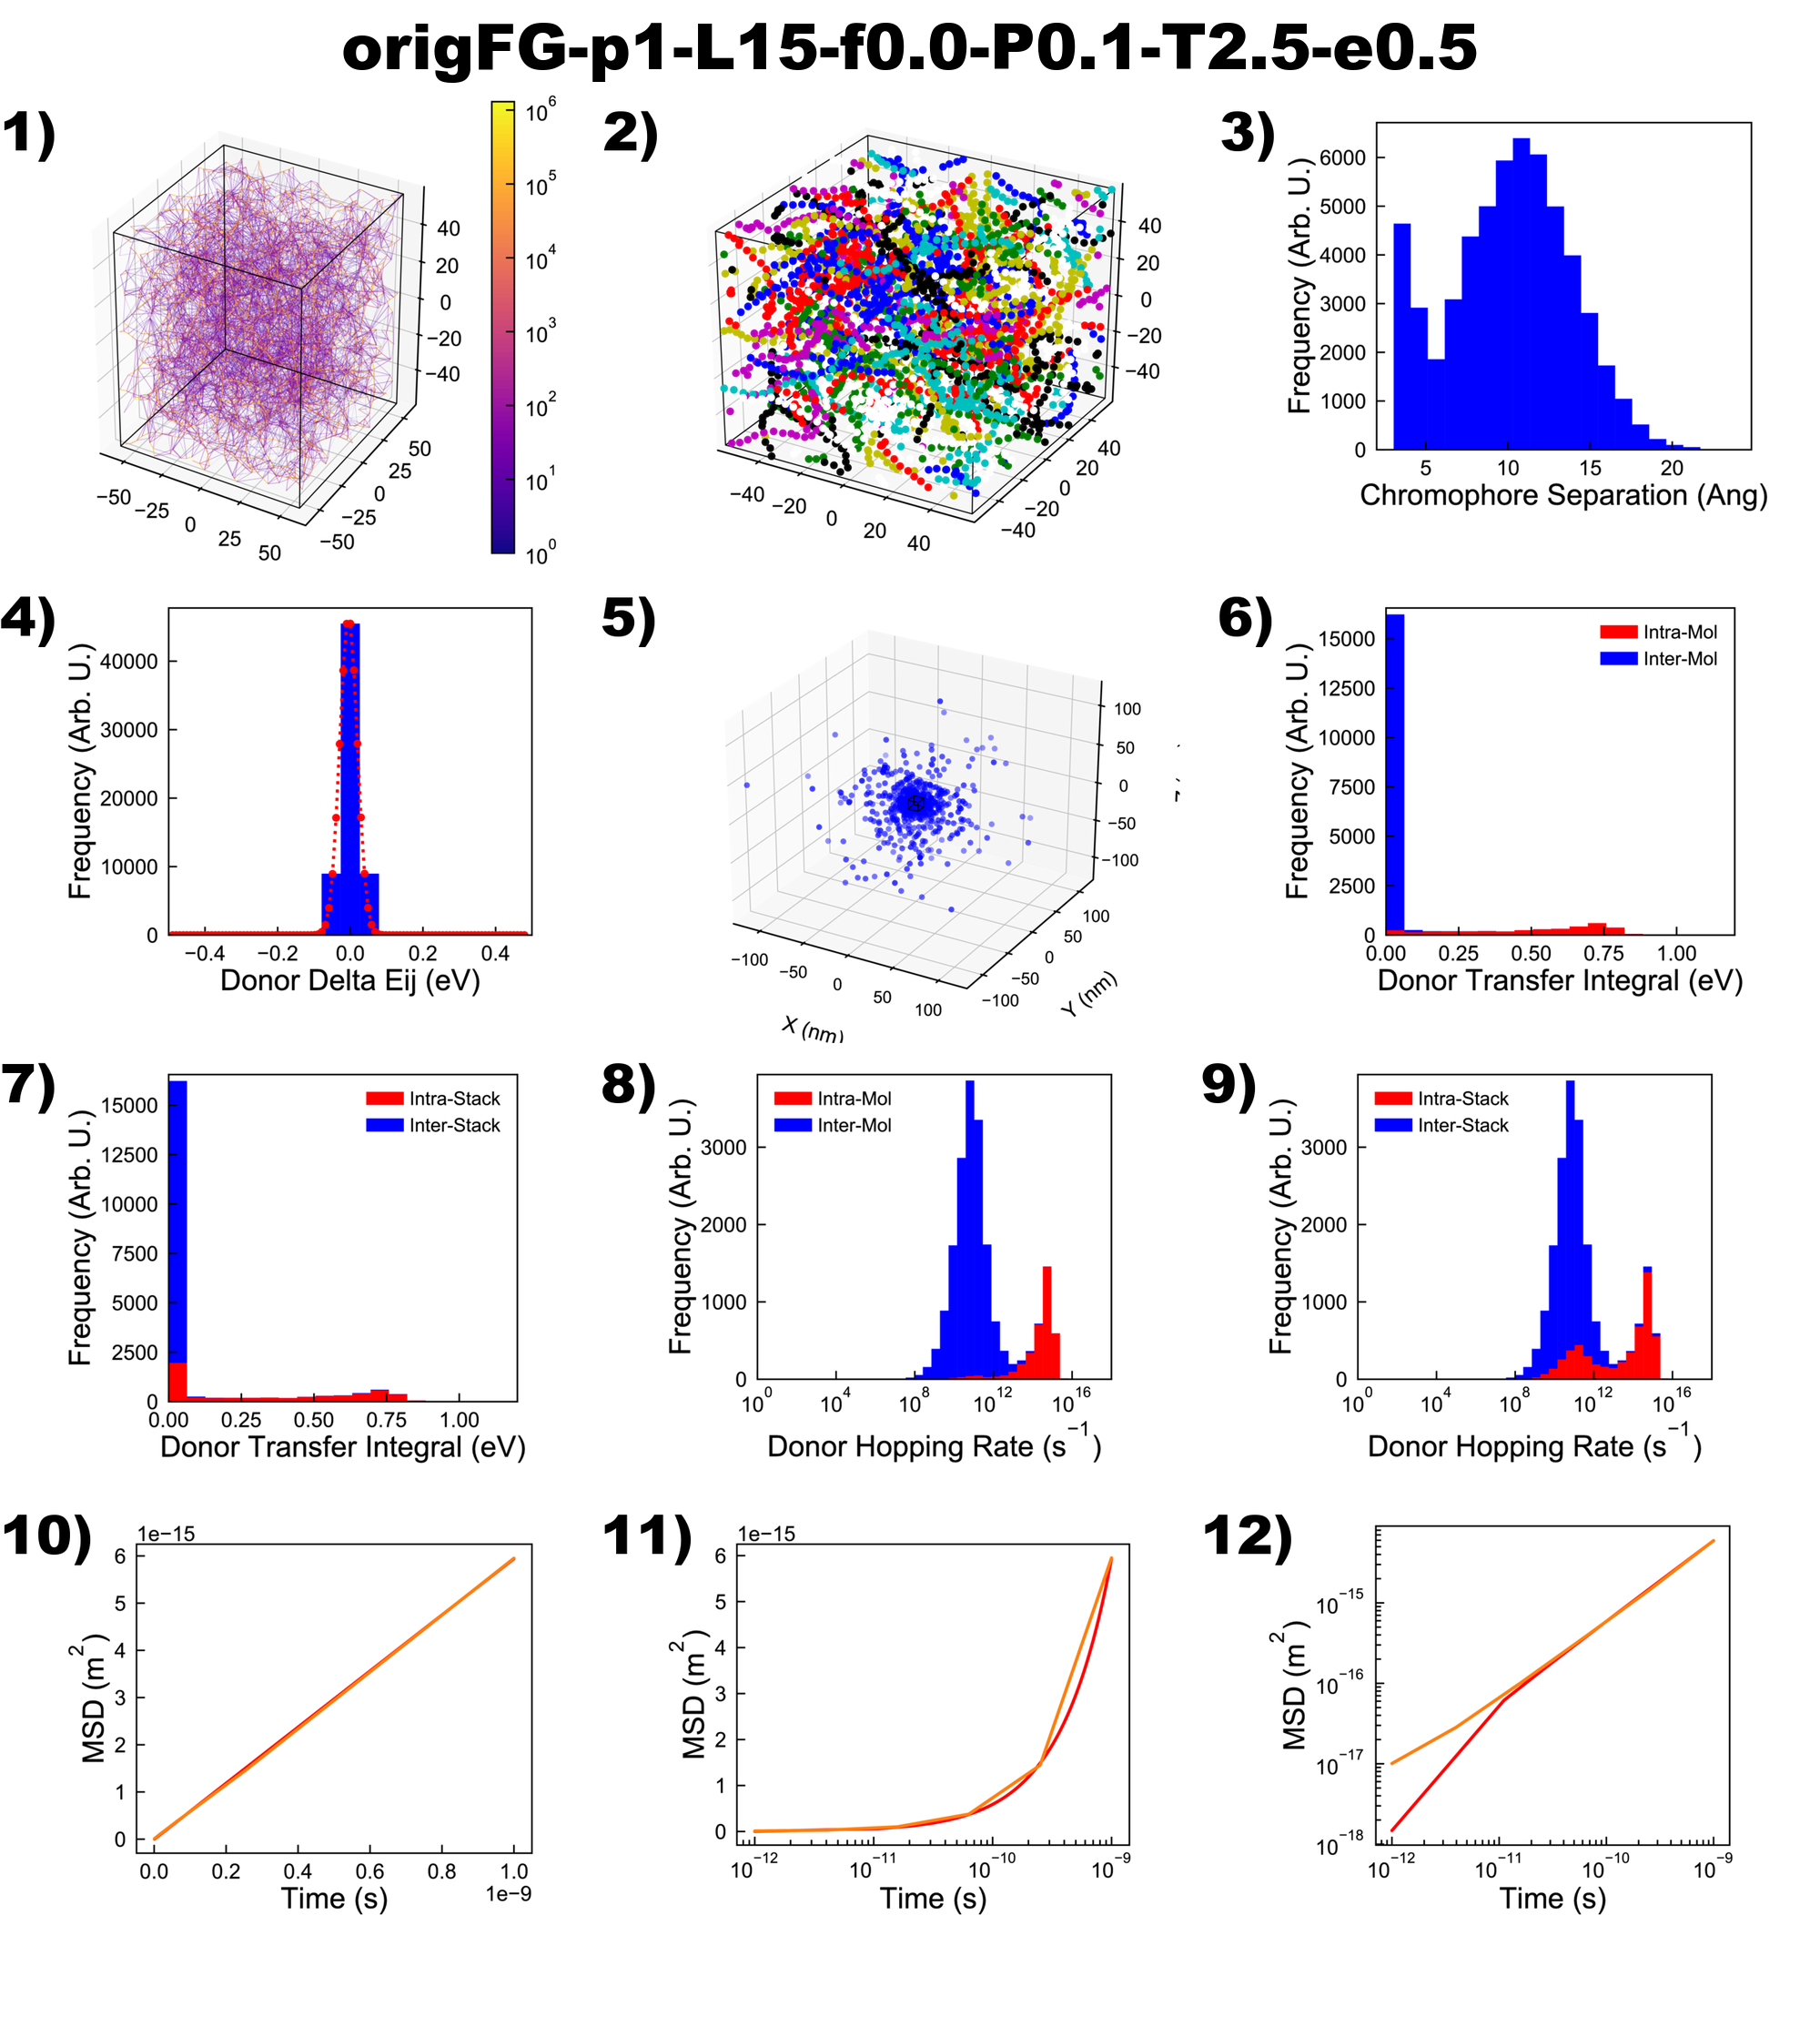
\includegraphics[width=\textwidth]{Figures/origFG-p1-L15-f0.0-P0.1-T2.5-e0.5.png}
    \caption{   1) Chromophore connectivity network, 
                2) Location of `stacks', 
                3) Distribution of connected chromophore separations (defines stacks),
                4) Density of states of Frontier molecular orbital (delta Eij),
                5) KMC Carrier termination locations (defines anisotropy),
                6) Histogram of molecular transfer integrals,
                7) Histogram of stack transfer integrals,
                8) Histogram of molecular hopping rates,
                9) Histogram of stack hopping rates,
                10) Linear MSD plot,
                11) Semi-log-x MSD plot,
                12) Logarithmic MSD plot.}
	\label{fig:UneqlT2.5}
\end{figure}


\clearpage

\subsection{New (Equilibrated) Results}

\begin{figure}[h]\centering
	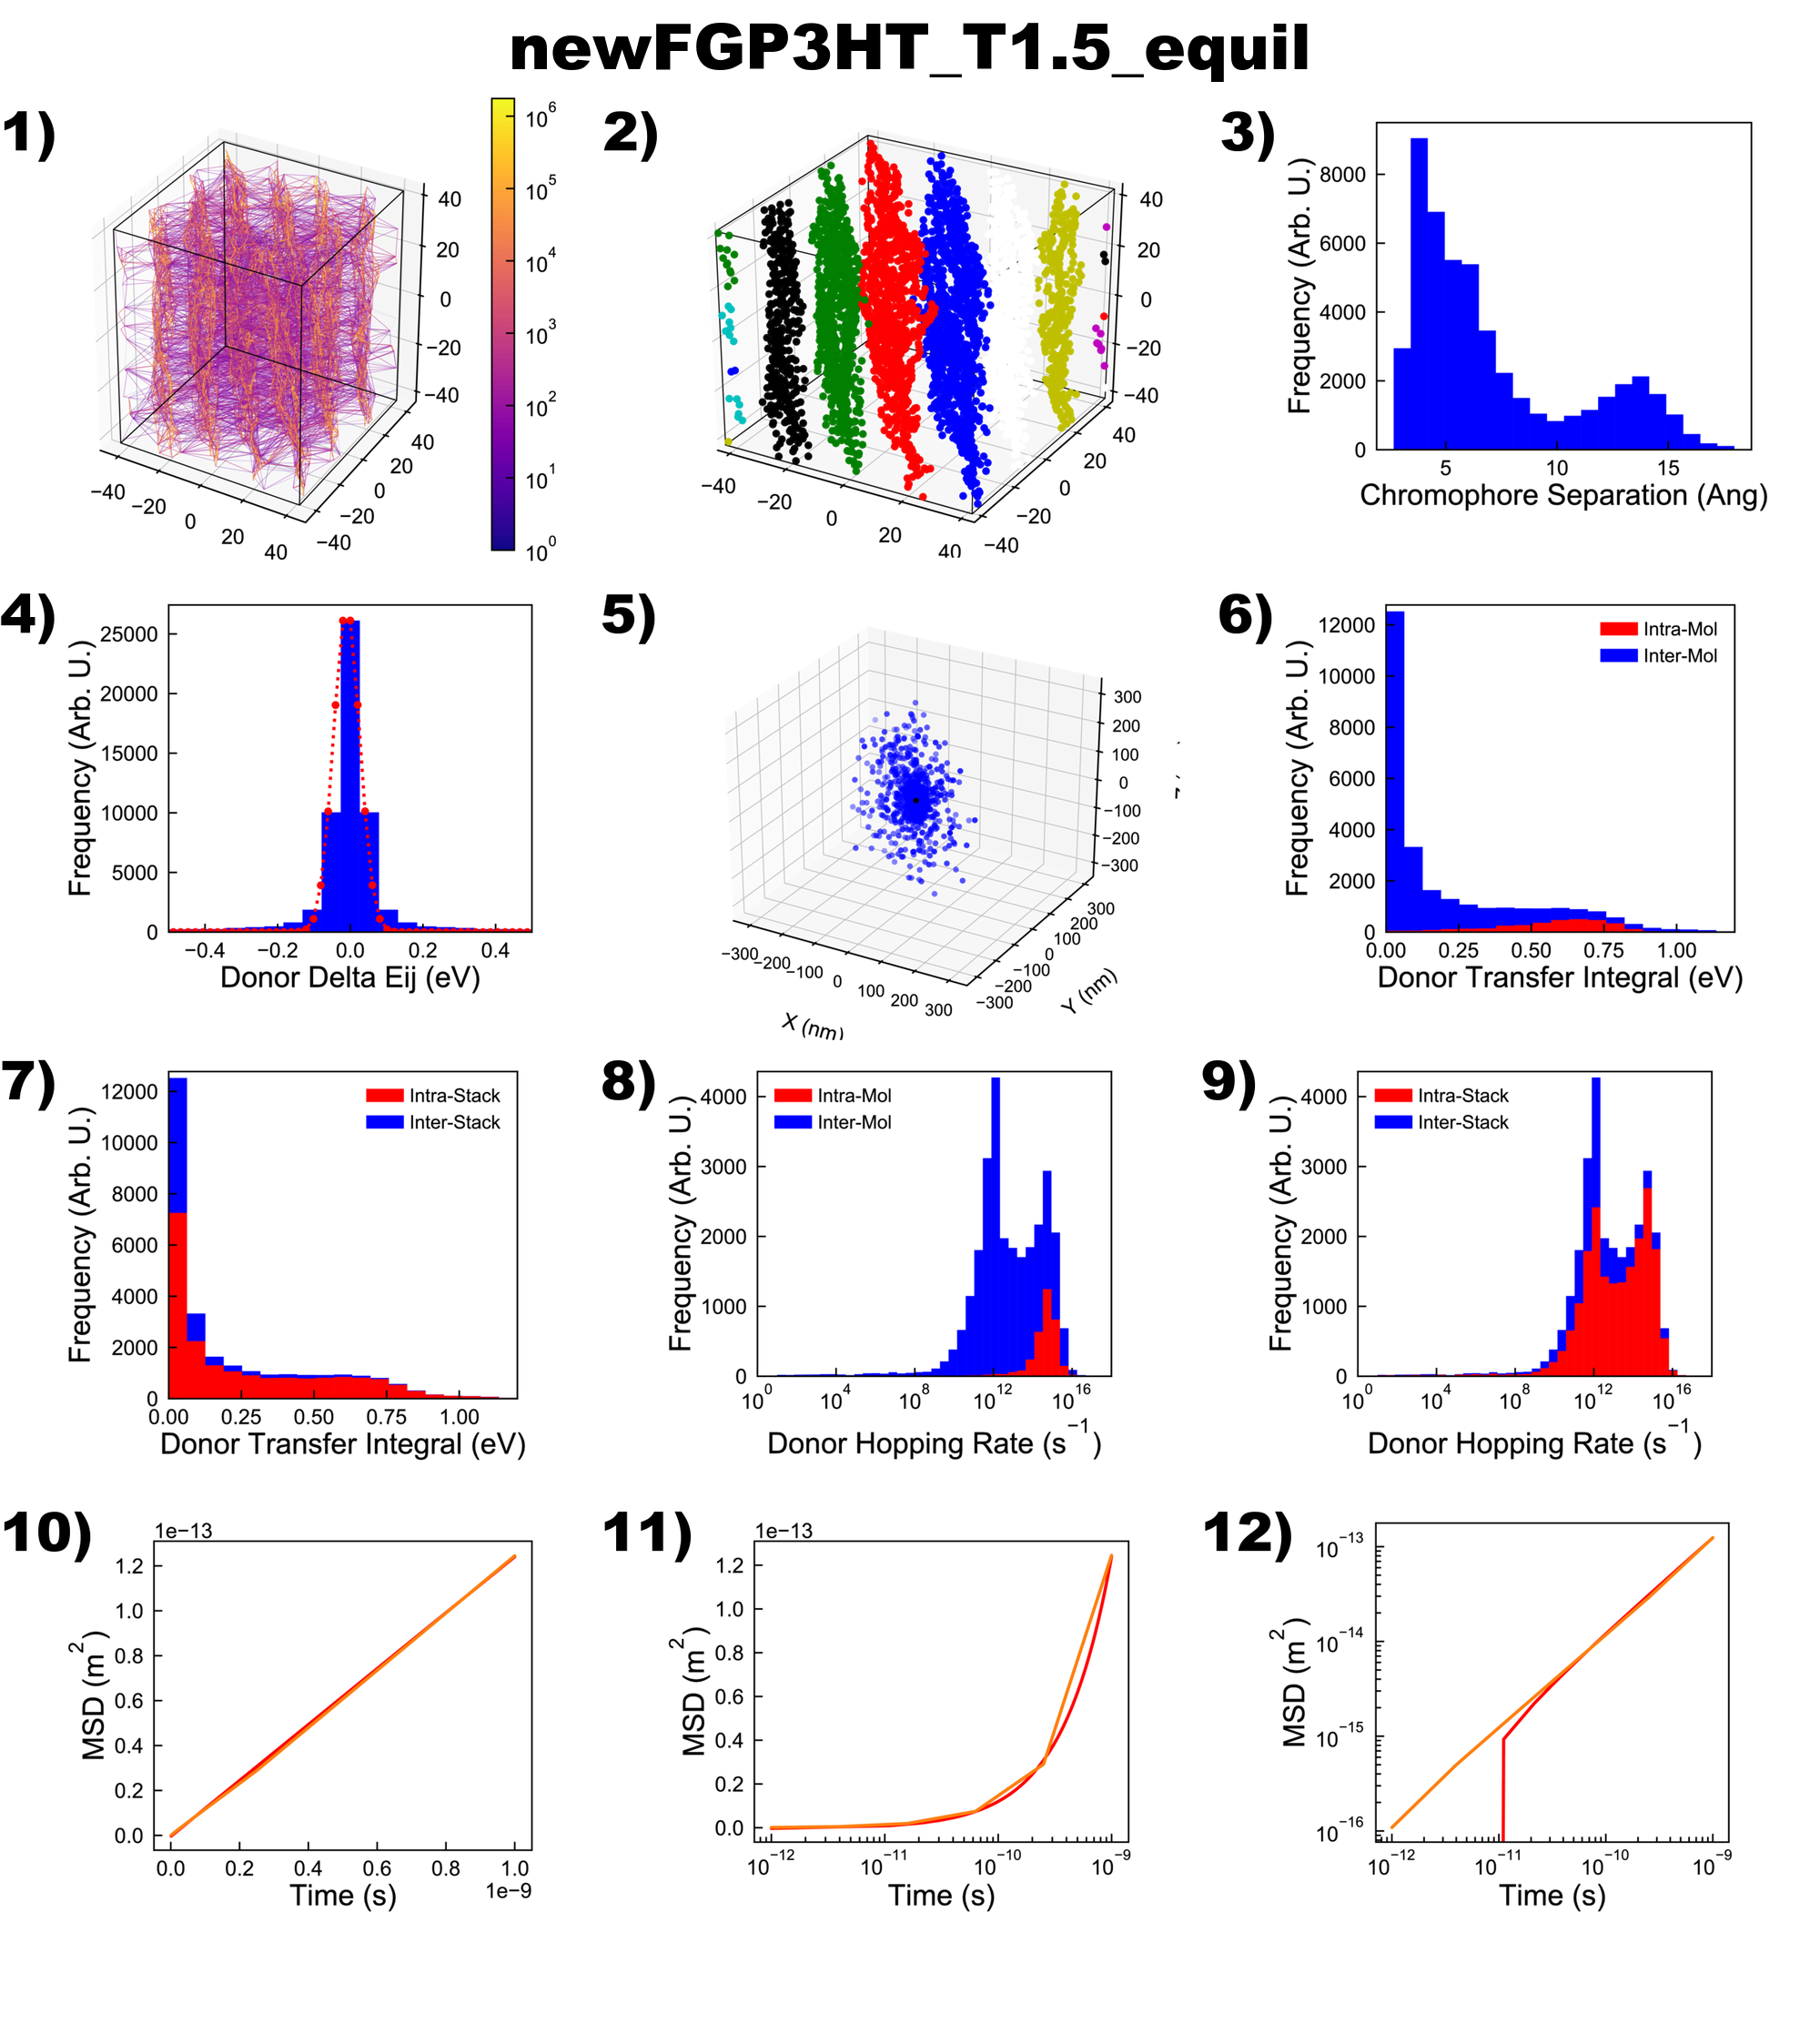
\includegraphics[width=0.80\textwidth]{Figures/newFGP3HT_T1.5_equil.png}
    \caption{   1) Chromophore connectivity network, 
                2) Location of `stacks', 
                3) Distribution of connected chromophore separations (defines stacks),
                4) Density of states of Frontier molecular orbital (delta Eij),
                5) KMC Carrier termination locations (defines anisotropy),
                6) Histogram of molecular transfer integrals,
                7) Histogram of stack transfer integrals,
                8) Histogram of molecular hopping rates,
                9) Histogram of stack hopping rates,
                10) Linear MSD plot,
                11) Semi-log-x MSD plot,
                12) Logarithmic MSD plot.}
	\label{fig:EqlT1.5}
\end{figure}


\begin{figure}[h]\centering
	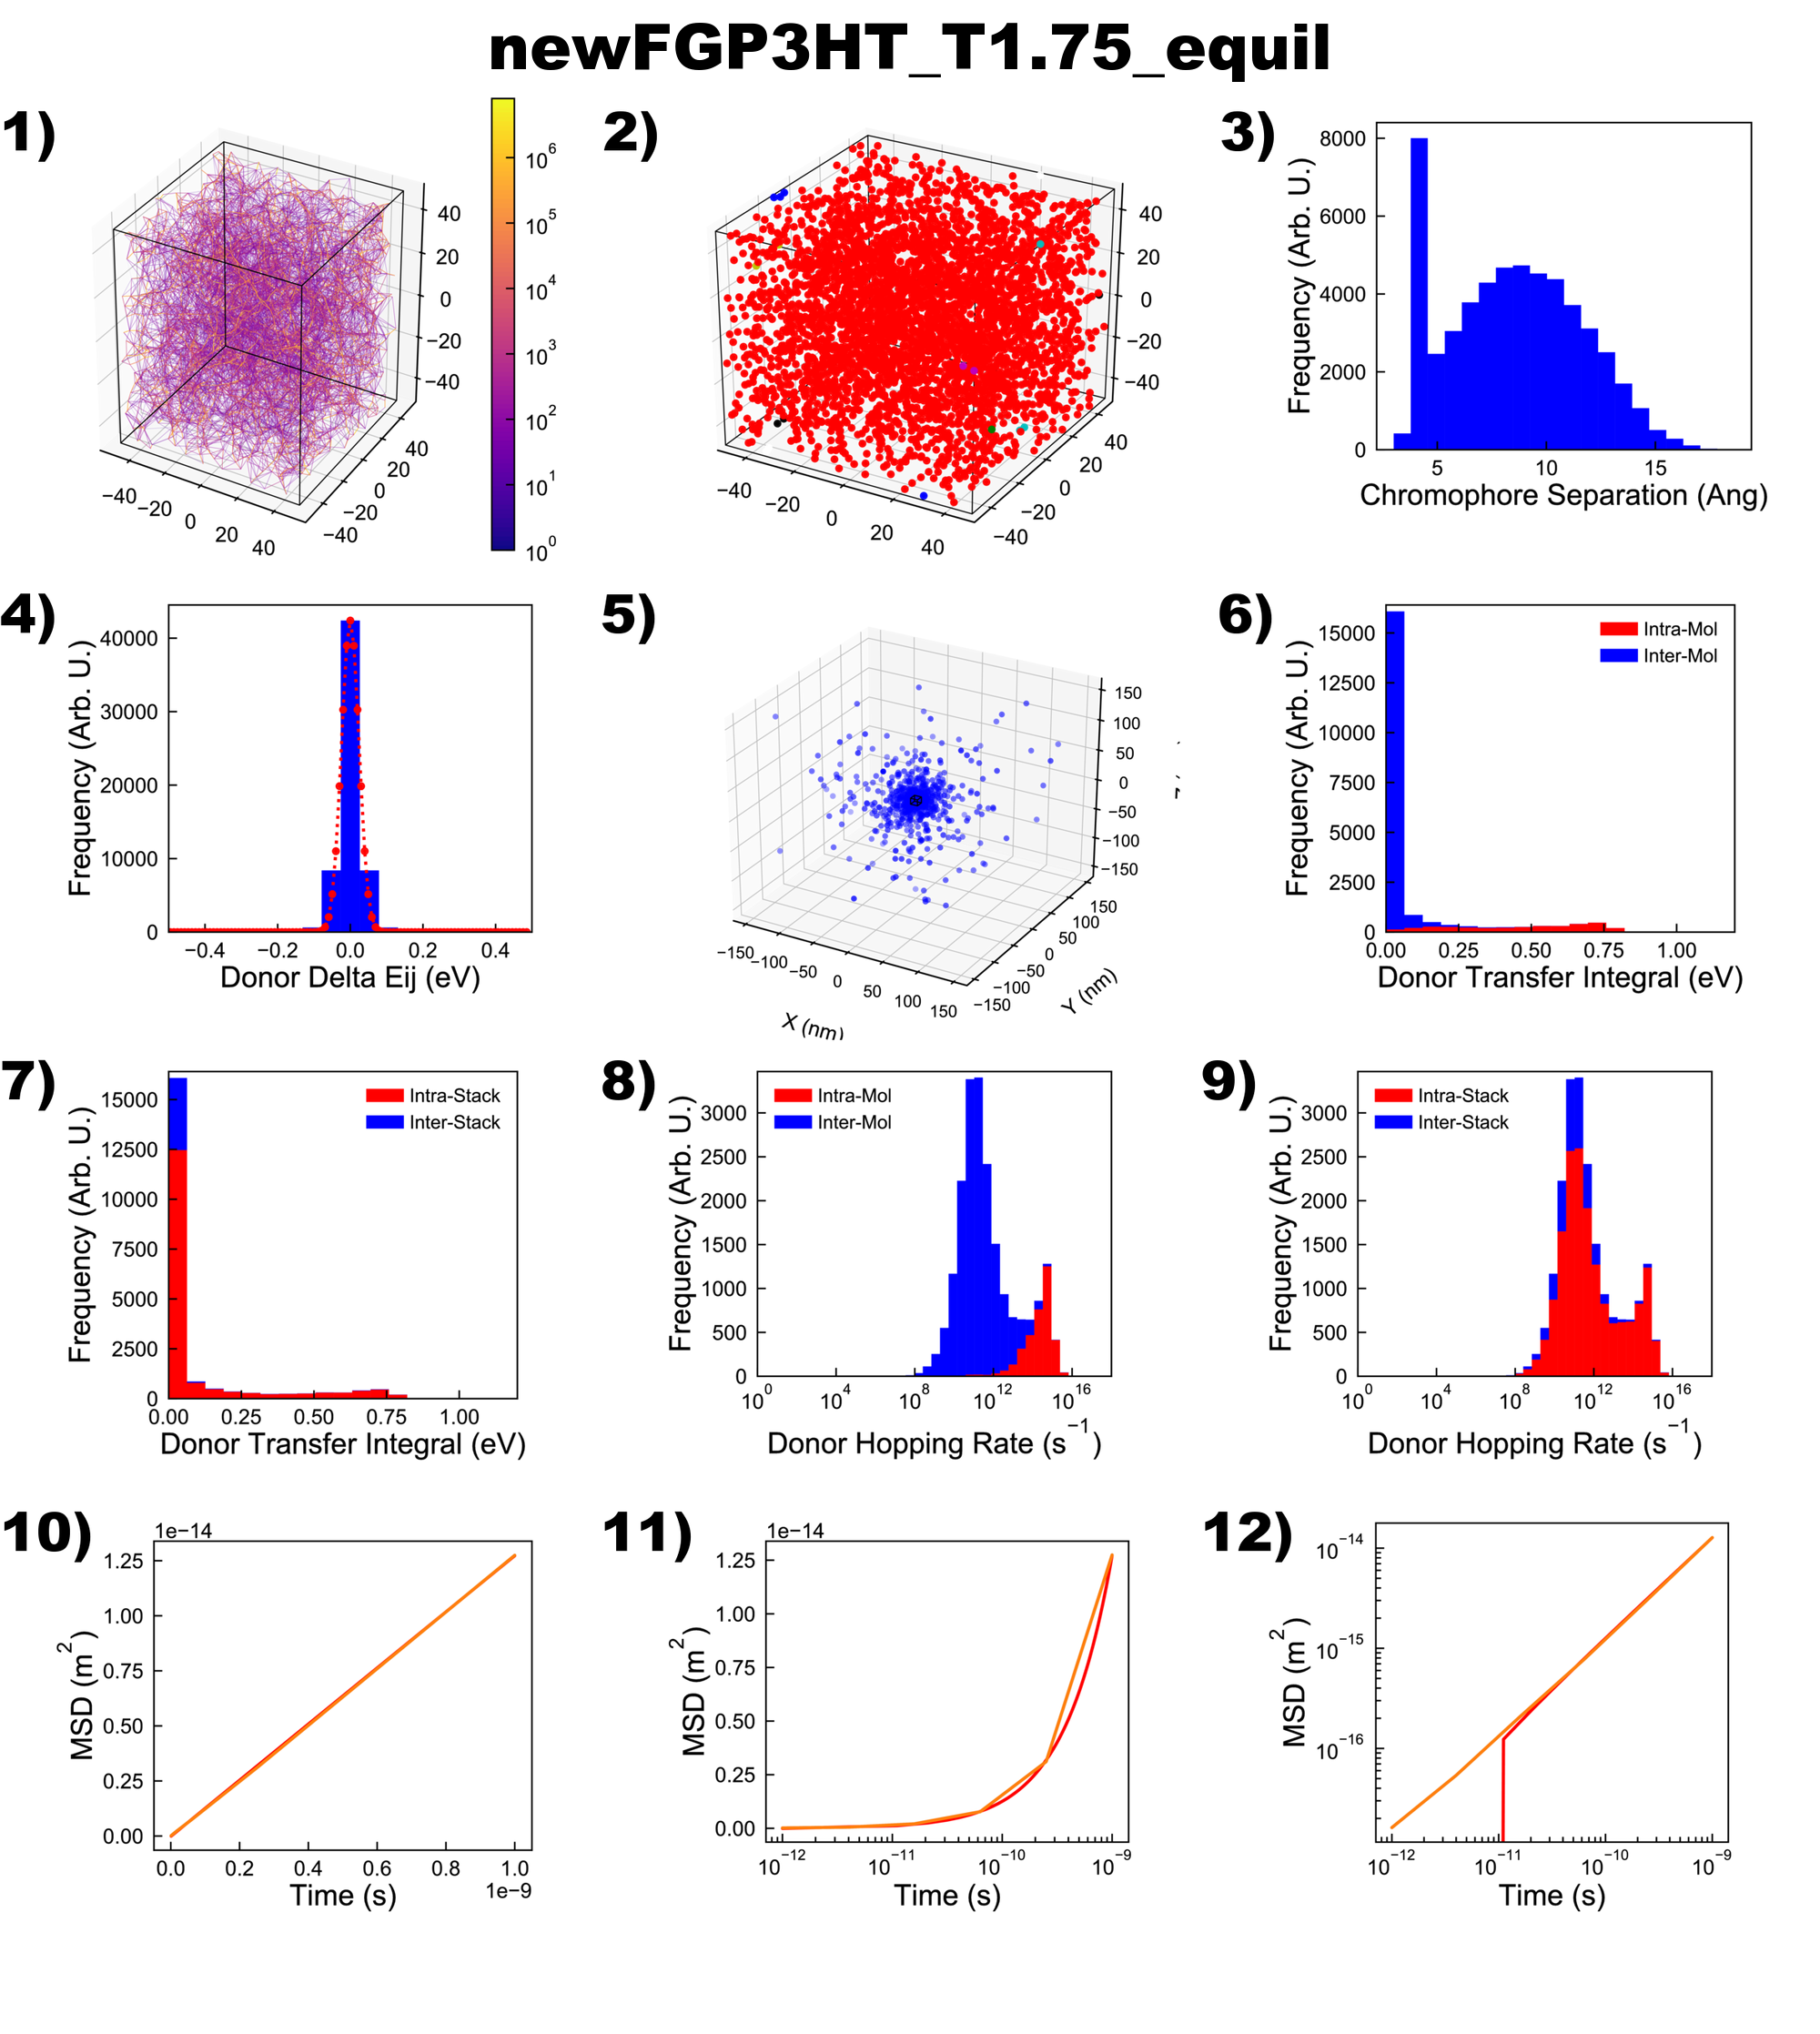
\includegraphics[width=\textwidth]{Figures/newFGP3HT_T1.75_equil.png}
    \caption{   1) Chromophore connectivity network, 
                2) Location of `stacks', 
                3) Distribution of connected chromophore separations (defines stacks),
                4) Density of states of Frontier molecular orbital (delta Eij),
                5) KMC Carrier termination locations (defines anisotropy),
                6) Histogram of molecular transfer integrals,
                7) Histogram of stack transfer integrals,
                8) Histogram of molecular hopping rates,
                9) Histogram of stack hopping rates,
                10) Linear MSD plot,
                11) Semi-log-x MSD plot,
                12) Logarithmic MSD plot.}
	\label{fig:EqlT1.75}
\end{figure}


\begin{figure}[h]\centering
	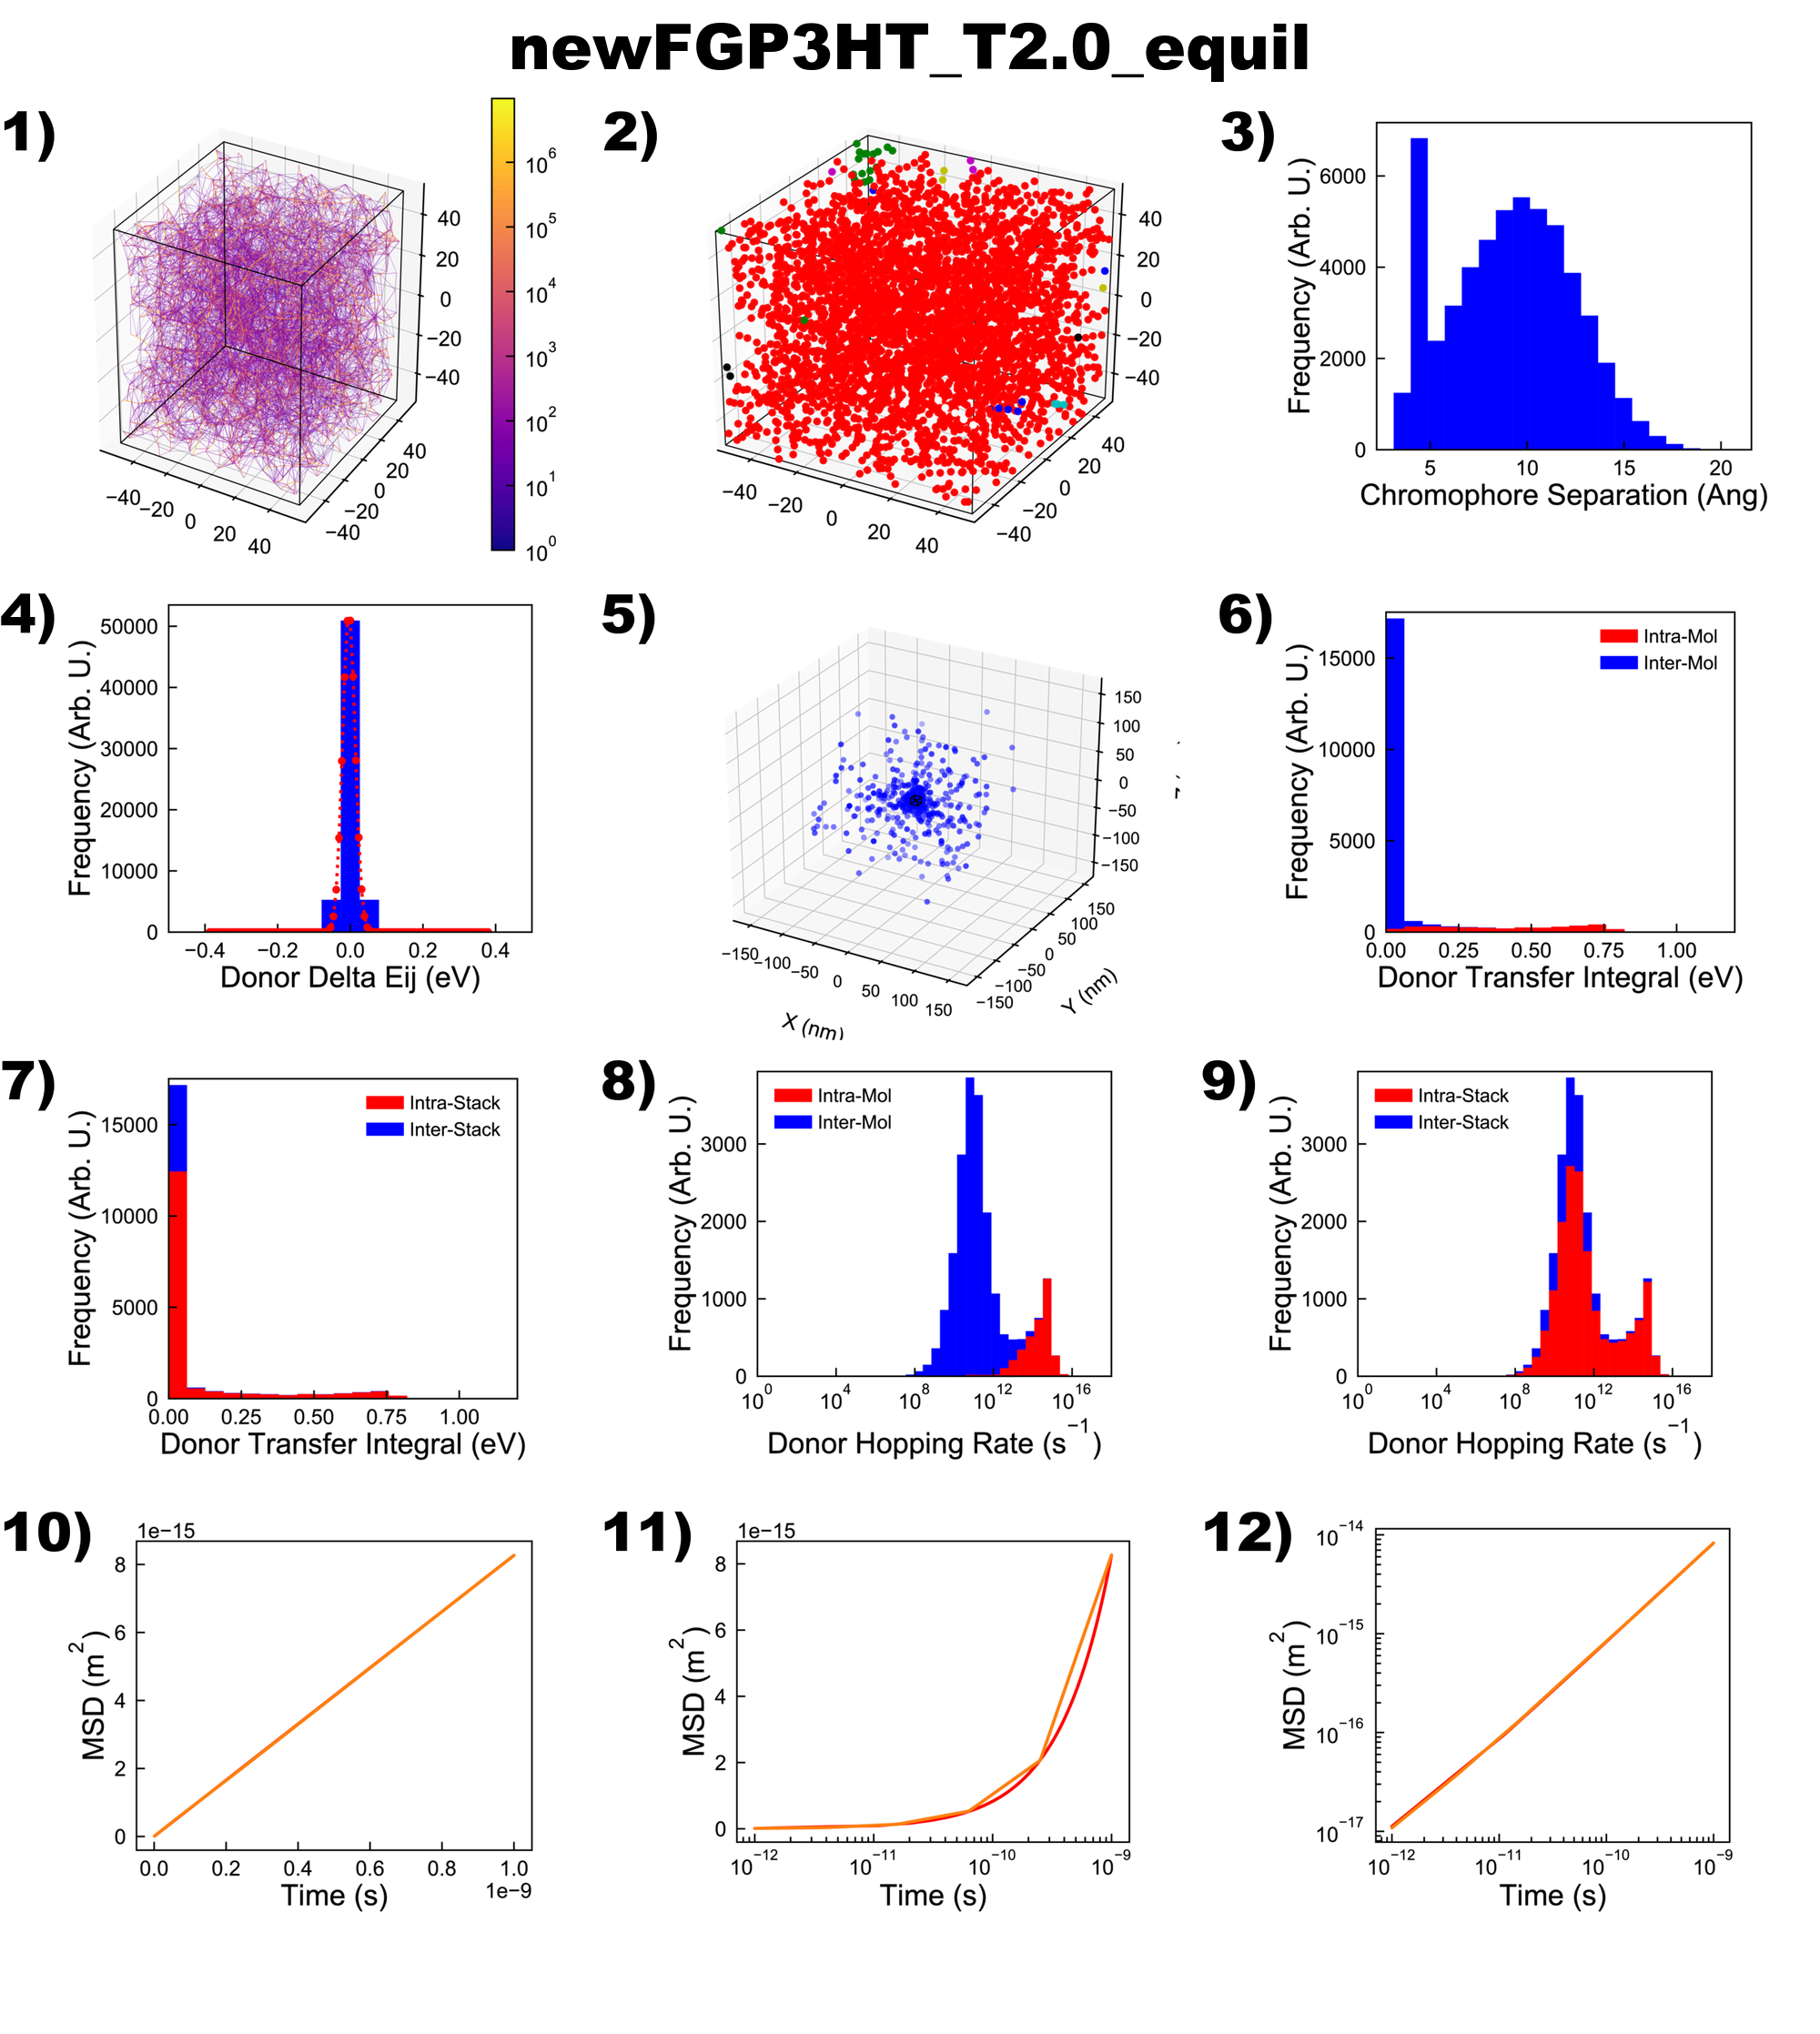
\includegraphics[width=\textwidth]{Figures/newFGP3HT_T2.0_equil.png}
    \caption{   1) Chromophore connectivity network, 
                2) Location of `stacks', 
                3) Distribution of connected chromophore separations (defines stacks),
                4) Density of states of Frontier molecular orbital (delta Eij),
                5) KMC Carrier termination locations (defines anisotropy),
                6) Histogram of molecular transfer integrals,
                7) Histogram of stack transfer integrals,
                8) Histogram of molecular hopping rates,
                9) Histogram of stack hopping rates,
                10) Linear MSD plot,
                11) Semi-log-x MSD plot,
                12) Logarithmic MSD plot.}
	\label{fig:EqlT2.0}
\end{figure}


\begin{figure}[h]\centering
	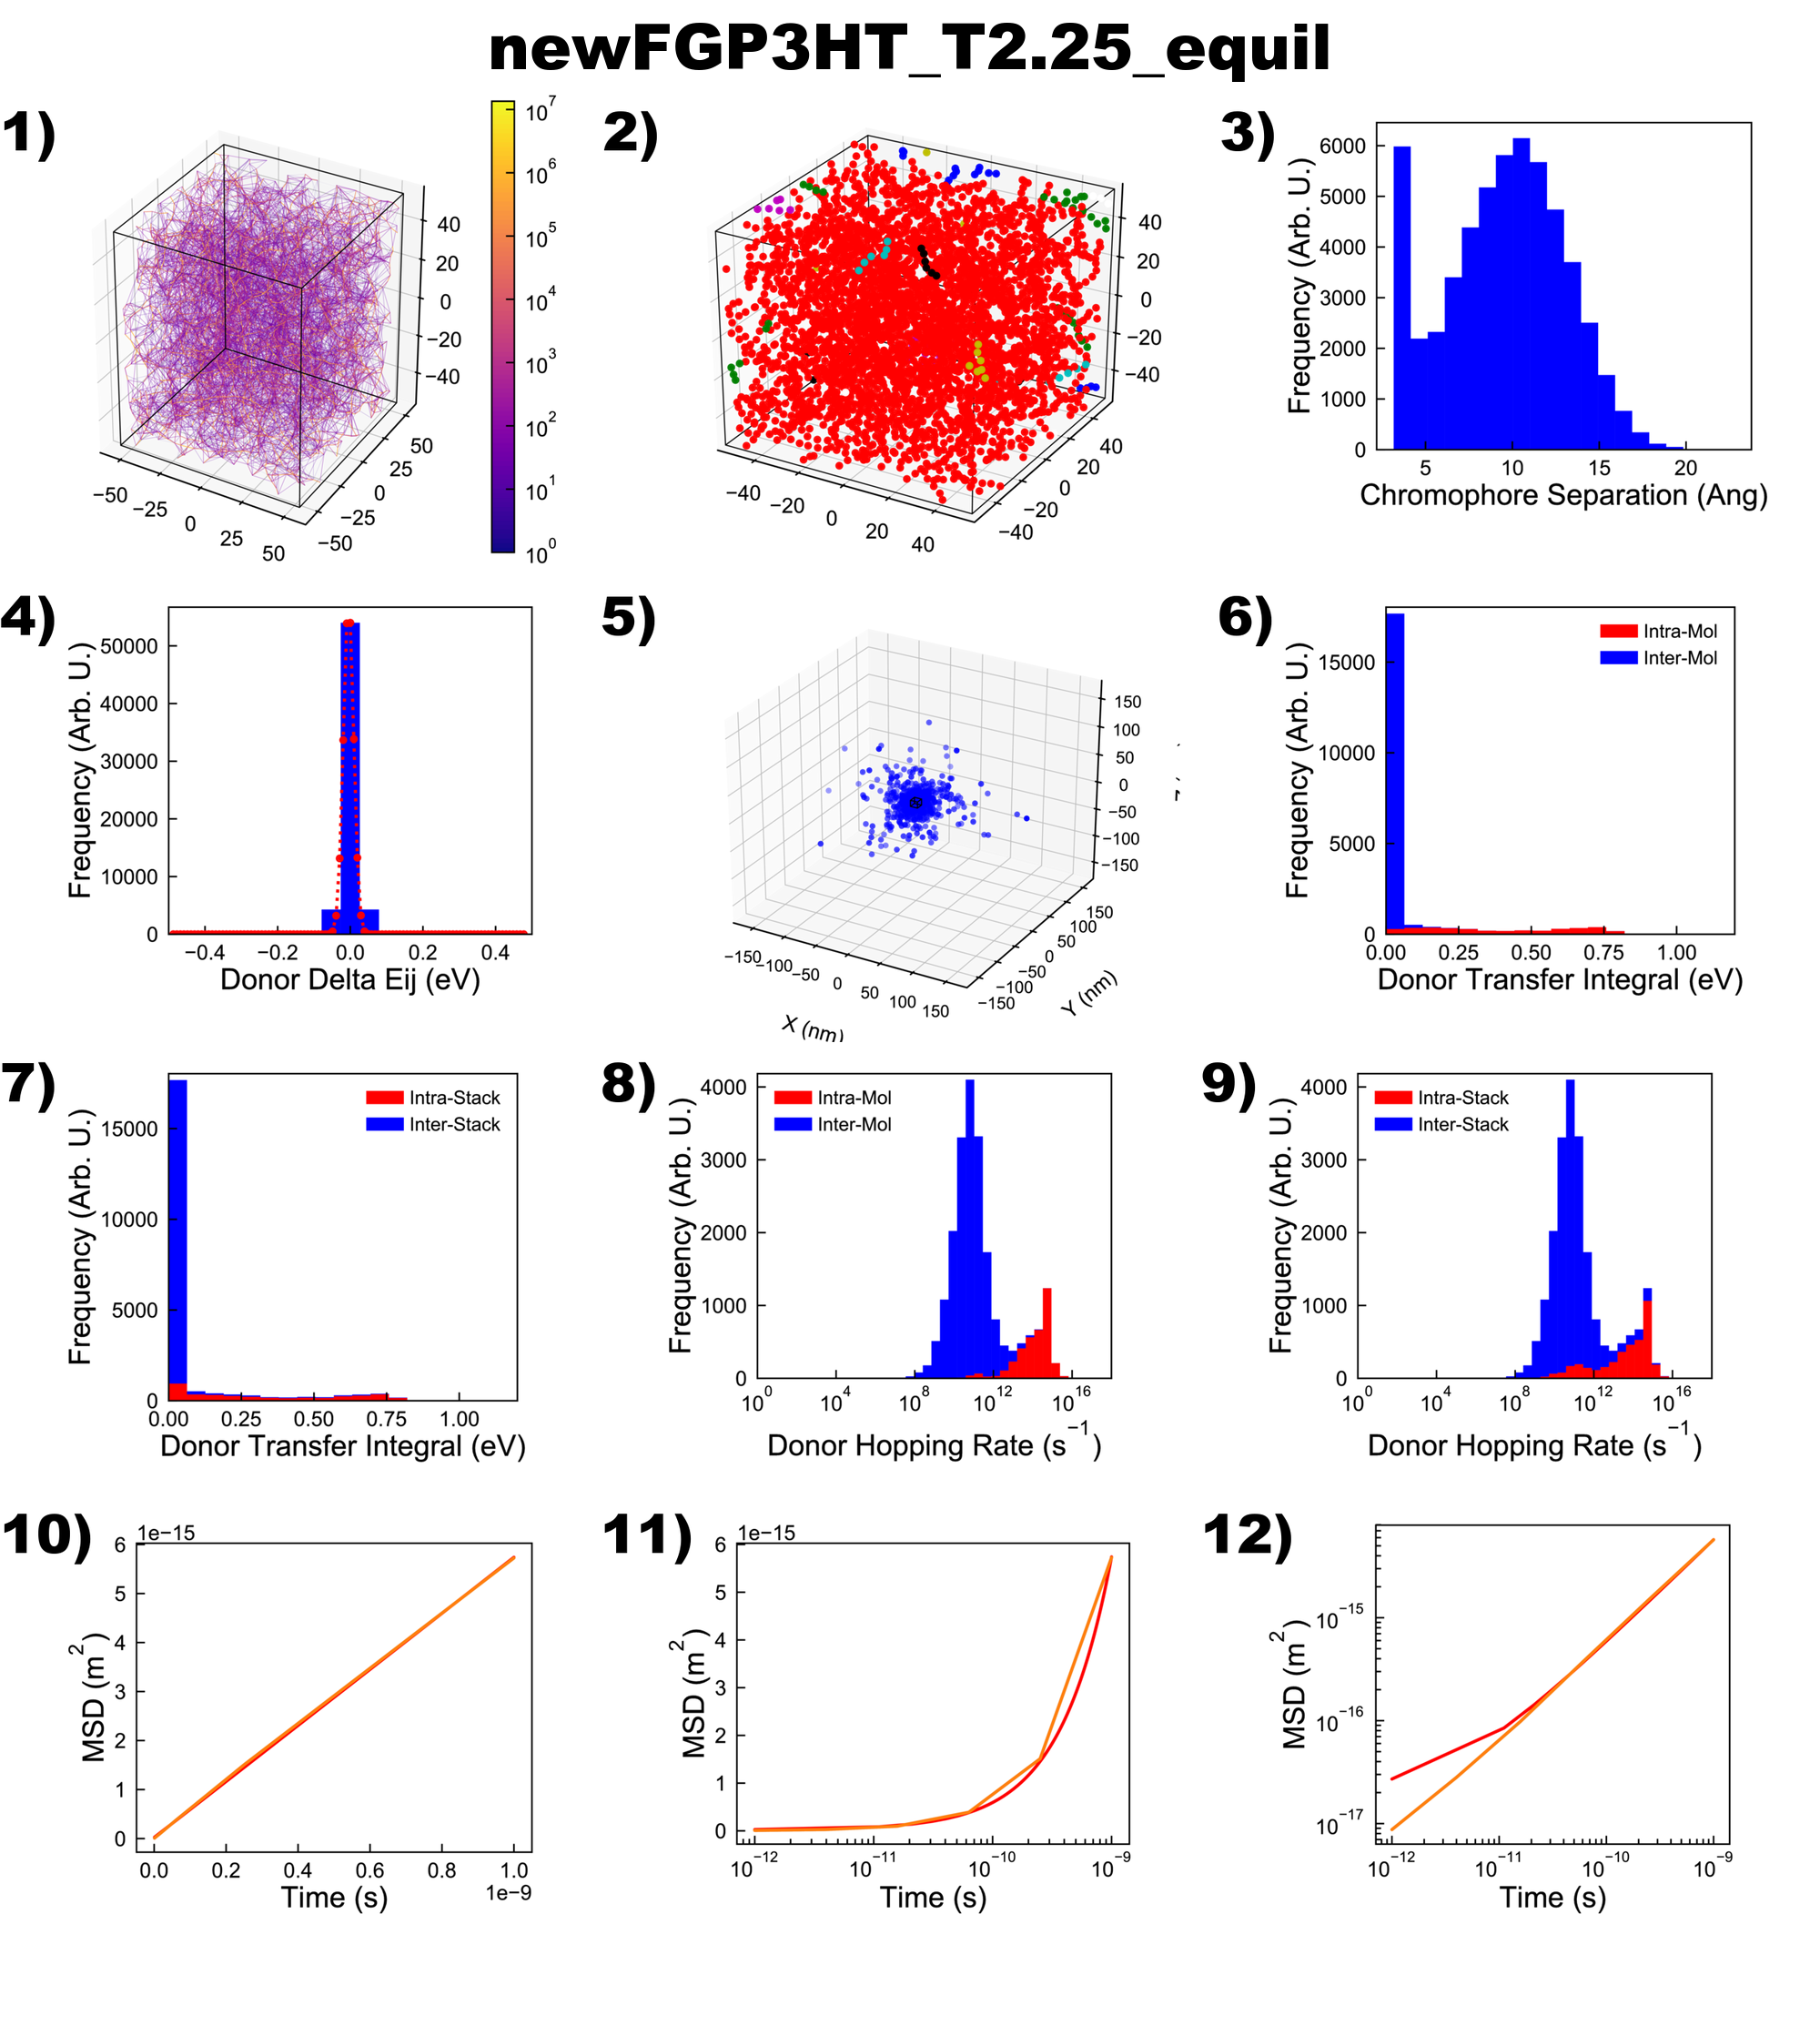
\includegraphics[width=\textwidth]{Figures/newFGP3HT_T2.25_equil.png}
    \caption{   1) Chromophore connectivity network, 
                2) Location of `stacks', 
                3) Distribution of connected chromophore separations (defines stacks),
                4) Density of states of Frontier molecular orbital (delta Eij),
                5) KMC Carrier termination locations (defines anisotropy),
                6) Histogram of molecular transfer integrals,
                7) Histogram of stack transfer integrals,
                8) Histogram of molecular hopping rates,
                9) Histogram of stack hopping rates,
                10) Linear MSD plot,
                11) Semi-log-x MSD plot,
                12) Logarithmic MSD plot.}
	\label{fig:EqlT2.25}
\end{figure}


\begin{figure}[h]\centering
	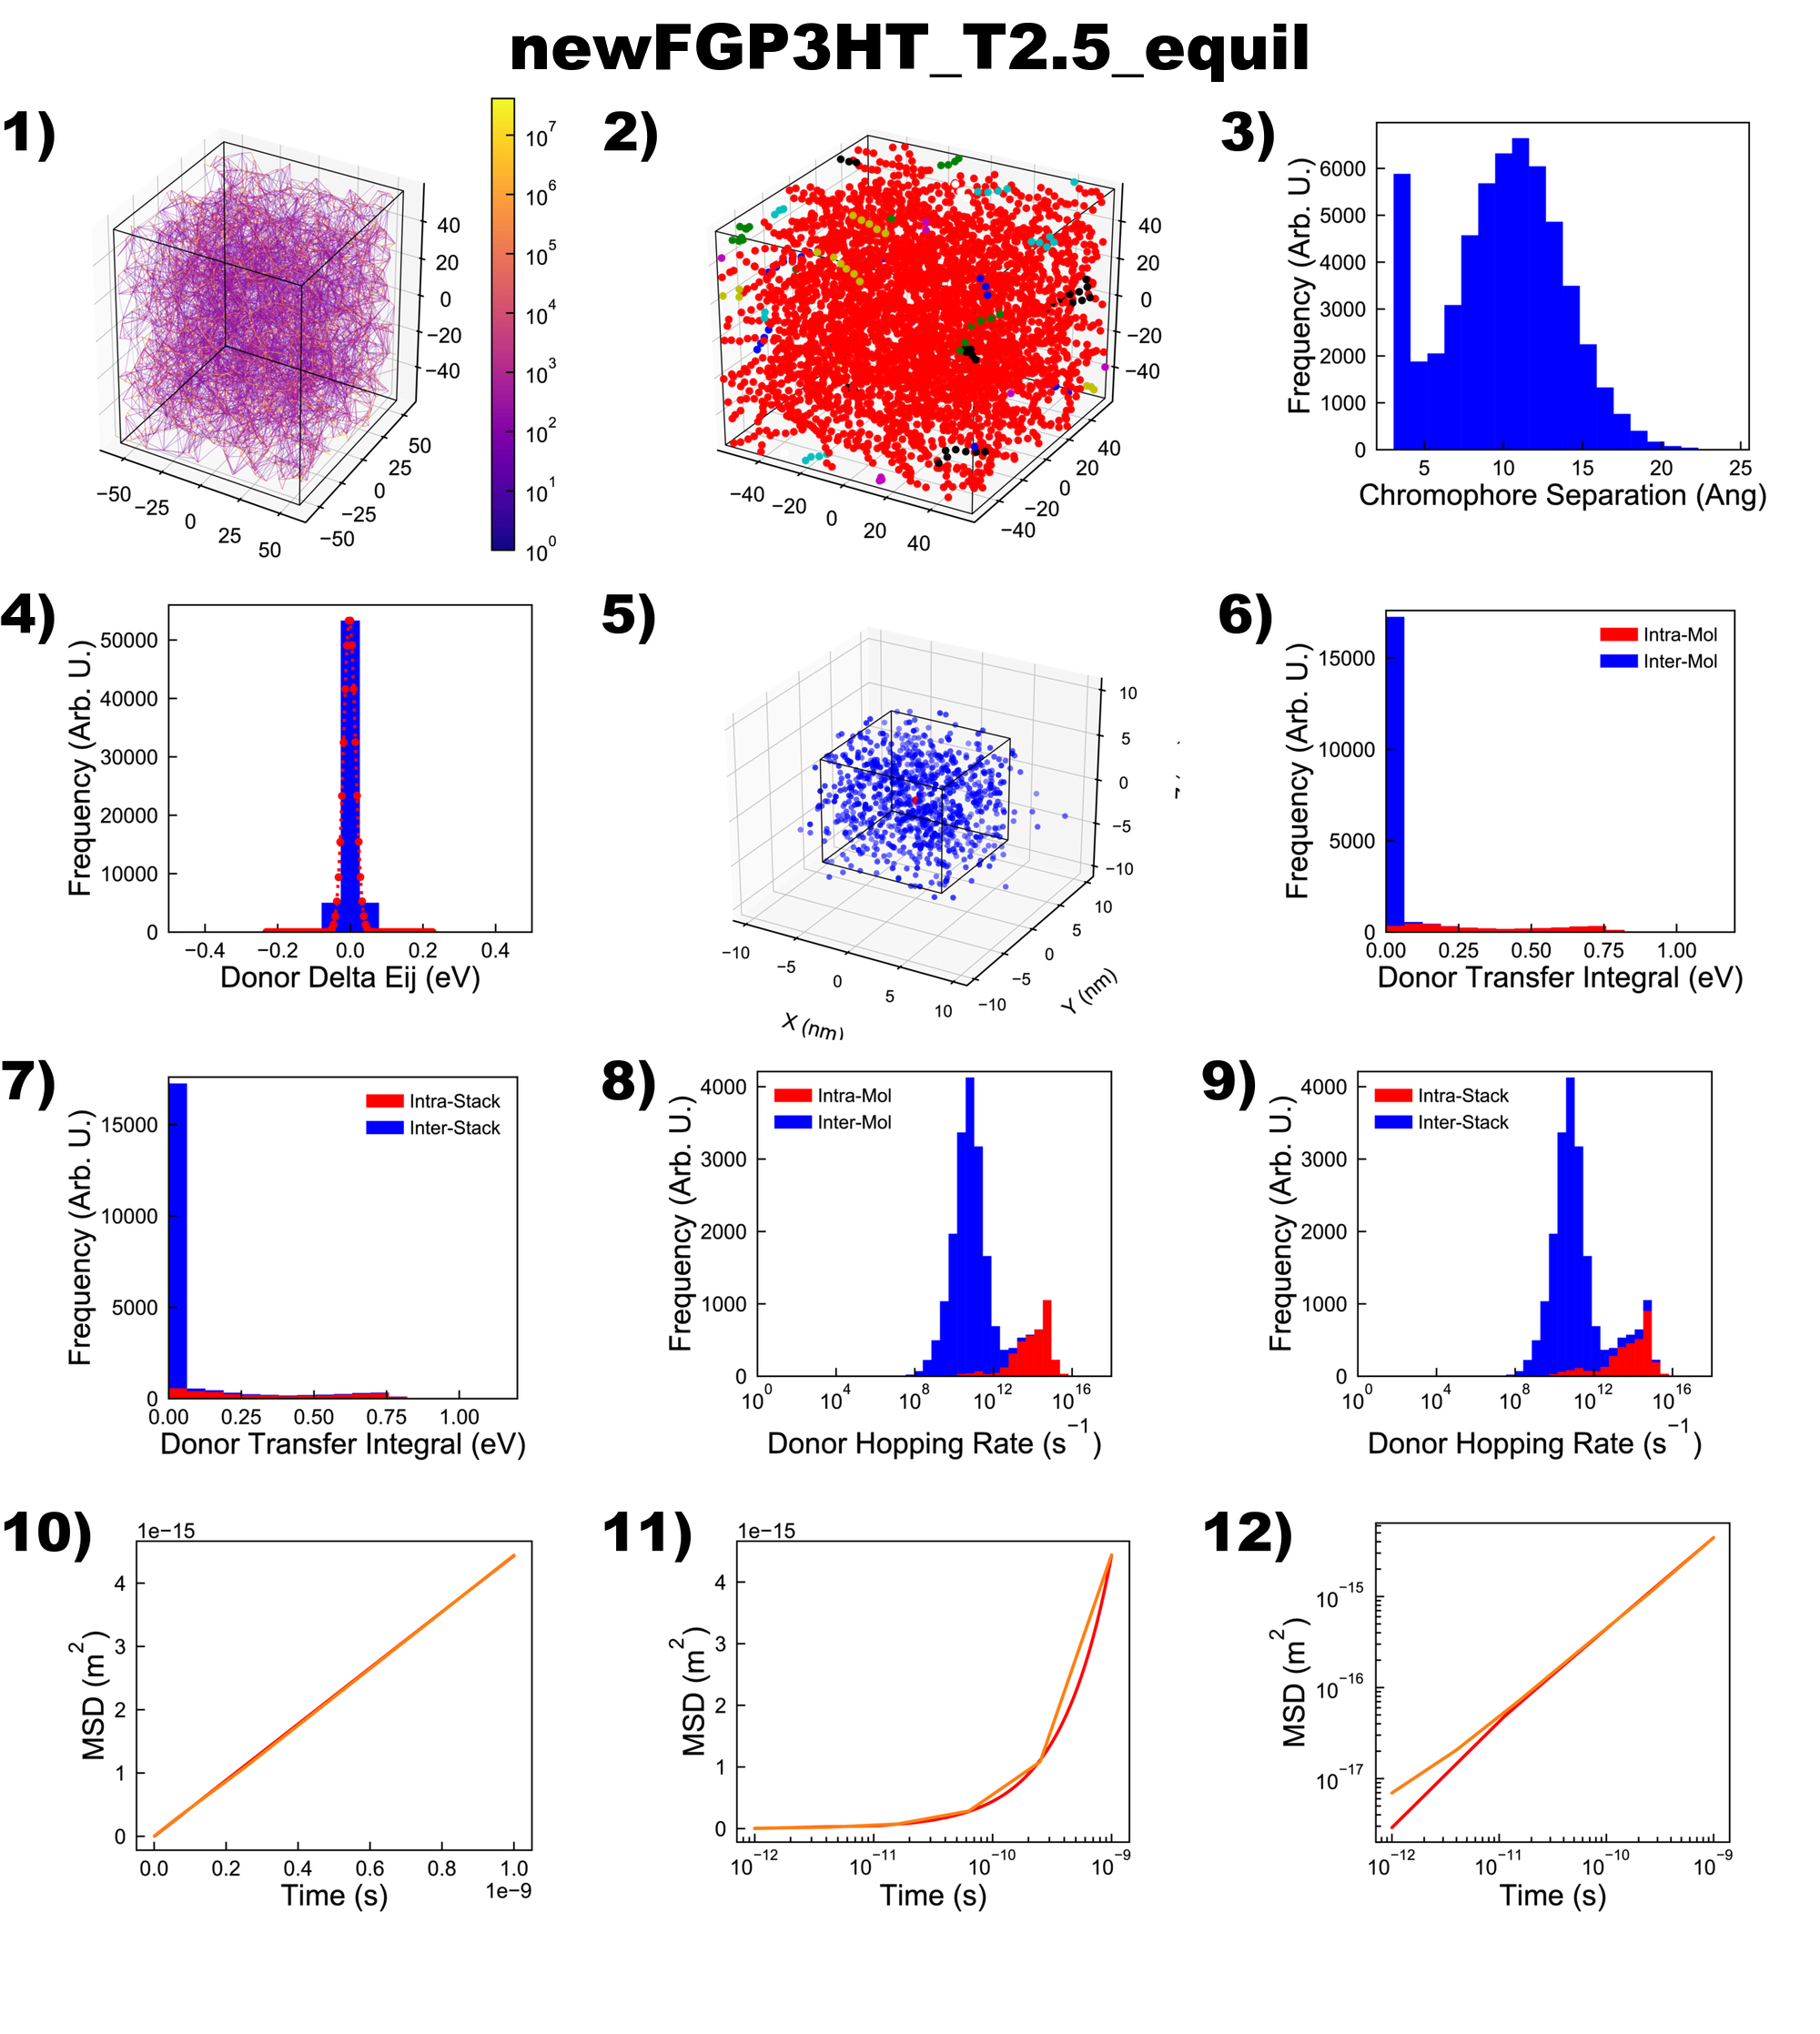
\includegraphics[width=\textwidth]{Figures/newFGP3HT_T2.5_equil.png}
    \caption{   1) Chromophore connectivity network, 
                2) Location of `stacks', 
                3) Distribution of connected chromophore separations (defines stacks),
                4) Density of states of Frontier molecular orbital (delta Eij),
                5) KMC Carrier termination locations (defines anisotropy),
                6) Histogram of molecular transfer integrals,
                7) Histogram of stack transfer integrals,
                8) Histogram of molecular hopping rates,
                9) Histogram of stack hopping rates,
                10) Linear MSD plot,
                11) Semi-log-x MSD plot,
                12) Logarithmic MSD plot.}
	\label{fig:EqlT2.5}
\end{figure}


\bibliography{refs}
\bibliographystyle{unsrt}


\end{document}
